\documentclass{article}

% Language setting
\usepackage[english]{babel}

% Set page size and margins
\usepackage[a4paper,top=2cm,bottom=2cm,left=3cm,right=3cm,marginparwidth=1.75cm]{geometry}

% Useful packages
\usepackage{amsmath}
\usepackage{amssymb}
\usepackage{graphicx}
\usepackage{tikz}
\usetikzlibrary{positioning}
\usepackage[colorlinks=true, allcolors=blue]{hyperref}
\usepackage{algpseudocode}
\usepackage{algorithm}

% Shaded derivation blocks
\usepackage{xcolor}
\usepackage{framed}
\definecolor{shadecolor}{gray}{0.95}
\newenvironment{derivation}{\begin{snugshade}\noindent\textit{Derivation.}\ }{\end{snugshade}}
\newenvironment{notebox}{\begin{snugshade}\noindent\textit{Note.}\ }{\end{snugshade}}
\newtheorem{definition}{Definition}


\setlength{\parindent}{0pt}
\setlength{\parskip}{0.5em}

\title{AML Summary}
\author{Lukas Diebold}

\begin{document}
\begin{titlepage}
    \centering
    {\Huge AML Summary\par}
    \vspace{0.5cm}
    {\Large Advanced Machine Learning Lecture at ETH\par}
    \vspace{2cm}
    {\large Lukas Diebold\par}
    \vfill
    {\large \today\par}
\end{titlepage}

\section*{Disclaimer}
These notes are based on the Advanced Machine Learning lecture at ETH. They are
provided without guarantees regarding correctness or completeness. Some images
are adapted from or taken directly from lecture slides and remain the property of
their respective owners. This document is intended for educational use.

\section*{Help Improve These Notes}
Feedback and contributions are welcome. If you spot mistakes, unclear passages,
or missing intuition, please reach out or open an issue so the notes can be
improved for everyone.

\newpage

\tableofcontents
\newpage

\section{Math Preliminaries}
\textbf{Gibbs Distribution}
The Gibbs distribution is a probability distribution that assigns likelihoods to states based on a cost function, with lower-cost states being more probable. Given a set of states $x \in \mathcal{X}$, a cost function $E(x)$, and an inverse temperature parameter $\beta > 0$, the Gibbs distribution is
$$
p(x)=\frac{1}{Z}e^{-\beta E(x)}
$$
where the partition function $Z$ ensures normalization
$$
Z=\sum_{x \in X} e^{-\beta E(x)}
$$

\subsection{Conditional distribution of a multivariate Gaussian}
\label{sec:cond-gaussian}
Let
\[
\begin{bmatrix} a \\ b \end{bmatrix} \sim \mathcal{N}\!\left(\begin{bmatrix} \mu_a \\ \mu_b \end{bmatrix},\
\begin{bmatrix}
\Sigma_{aa} & \Sigma_{ab} \\
\Sigma_{ba} & \Sigma_{bb}
\end{bmatrix}\right),
\]
where $\Sigma_{aa}$ and $\Sigma_{bb}$ are covariance blocks and $\Sigma_{ab} = \Sigma_{ba}^\top$. Then the conditional distribution of $a$ given $b$ is again Gaussian with
\[
\mathbb{E}[a\mid b] = \mu_a + \Sigma_{ab} \, \Sigma_{bb}^{-1} (b - \mu_b),\quad
\operatorname{Cov}(a\mid b) = \Sigma_{aa} - \Sigma_{ab} \, \Sigma_{bb}^{-1} \, \Sigma_{ba}.
\]
This identity underlies Gaussian process prediction, Bayesian linear regression posteriors, and Kalman filtering.

\begin{derivation}
Write the joint as a block Gaussian and use the Schur complement. The joint log-density (up to constants) is
\[
\ell(a,b) = \tfrac{1}{2}\begin{bmatrix} a-\mu_a \\ b-\mu_b \end{bmatrix}^{\!\top}
\begin{bmatrix}
\Sigma_{aa} & \Sigma_{ab} \\
\Sigma_{ba} & \Sigma_{bb}
\end{bmatrix}^{\!-1}
\begin{bmatrix} a-\mu_a \\ b-\mu_b \end{bmatrix}.
\]
Completing the square in $a$ (or applying the standard conditional Gaussian formula) yields
\[
\mathbb{E}[a\mid b] = \mu_a + \Sigma_{ab} \Sigma_{bb}^{-1}(b-\mu_b),\quad
\operatorname{Cov}(a\mid b) = \Sigma_{aa} - \Sigma_{ab} \Sigma_{bb}^{-1} \Sigma_{ba}.
\]
Equivalently, these follow from the block inversion identity and the Schur complement of $\Sigma_{bb}$.
\end{derivation}

\subsection{Schur complement}
\label{sec:schur-complement}
\begin{notebox}
For a block matrix $M = \begin{bmatrix} A & B \\ C & D \end{bmatrix}$ with $D$ invertible, the \textbf{Schur complement of $D$ in $M$} is
\[
S = A - B D^{-1} C.
\]
Key identities (when the required inverses exist):
\begin{itemize}
	\item Determinant: $\det(M) = \det(D)\, \det(S)$.
	\item Block inverse: $M^{-1} = \begin{bmatrix}
	S^{-1} & -S^{-1} B D^{-1} \\
	-D^{-1} C S^{-1} & D^{-1} + D^{-1} C S^{-1} B D^{-1}
	\end{bmatrix}$.
	\item If $M$ is symmetric positive (semi)definite and $D$ is invertible, then $S$ is also positive (semi)definite.
\end{itemize}
Symmetrically, if $A$ is invertible, the Schur complement of $A$ is $D - C A^{-1} B$. In Gaussian conditioning, $\operatorname{Cov}(a\mid b)$ equals the Schur complement of $\Sigma_{bb}$ in the joint covariance.
\end{notebox}
\section{Conceptual Foundation}

\subsection{What is Machine Learning?}

"ML is a mathematization of epistemolagy!". In philosophy, it is the science of knowledge, the science of what can be known. This is relevant, because in ML we are interested in systems that produce/generate knowledge. 

The goal is then to observe 'reality' and draw conclusions from the observations. This can be seen as a perception-action cycle. Where perception is the result of our observations (typically in a data space $\mathcal X$) and the actions are part of a hypothesis space. To go from the data space to the hypothesis class $\mathcal C$ we generally use an algorithm $A$. See Figure \ref{fig:overview_ml} for an overview.
\begin{figure}[htbp]
  \centering
  \includegraphics[width=0.8\textwidth]{images/aml_1.png}
  \caption{Overview ML}
  \label{fig:overview_ml}
\end{figure}

\textbf{Information processing} occurs when $|\mathcal X| \gg |\mathcal C|$. Taking the example of combinatorial optimization problems, $|\mathcal X|$ would be the space of weighted graphs, and we look for a color of the graph or something similar. Then $|\mathcal X| \approx K^{\binom{n}{2}}$ and $|\mathcal C| \approx e^{n \log n}$ so we obserge that $|\mathcal X|$ is much larger. 

\subsection{Conceptual foundation of inference}
\begin{enumerate}
    \item Perception of realits is mediated by data of senses/sensors
    \item Data are stochastic → porbabilistic
    \item Sensing restricts us to selected aspects of reality
    \item Humans interpret data by a huge reduction in degrees of freedom \\
    $\quad|x| \gg|e|$ (space of graphs $\gg$ space of colorings, cycles, spanning trees)
    \item Tuple (\{data \}, \{hypotheses \}) define models:
    $$
    \begin{aligned}
    \mathcal A: \mathcal X &\longrightarrow \mathcal C \\
    x &\longmapsto c= \mathcal A(x)
    \end{aligned}
    $$
    \item Experiments $\epsilon$ provide us with data
    \item Learning means interpreting $X$ w.r.t hypotheses $\mathcal C$
\end{enumerate}

\subsection{Artificial Intelligence}
Taking a high level view. We live in very high dimensional data, which we are not able to fully process. We use algorithms to make sense of the data, and this then informs our values, from this we get the following relation
$$
\text { Data} \longrightarrow \text{ Algorithms } \mathcal{A} \longrightarrow \text { Values }
$$
In epistemology, we differentiate between \textbf{deduction} and \textbf{induction}. Deduction is a form of reasoning in which the conclusion follows necessarily from the premises, while induction tries to generalize, that is, the conclusion goes beyond the premises and generally probabilistic. We can construct a model in which deduction and induction form a \textbf{feedback loop}, not two isolated methods. In simpler terms, on one side we try to formulate axioms from our observations (empirical data), and on the other side we then use these axioms and derive logical consequences from them. This is not anything new, and this cycle generally informs the model of "Theory, Experiment, Computation" in science. What has changed with ML/AI is that we're now in the era of non-parametric modeling.

\subsection{Extracting Value from Data - What is the problem?}

\begin{itemize}
    \item Algorithms that process inputs with noise compute random variables as outputs!
    \item Algorithms should compute typical solutions!
    \item When do algorithms generalize over noise/model mismatch?
    \item How can algorithms autonomously improve performance?
\end{itemize}

\subsection{What does Generalization mean?}

\begin{itemize}
    \item Out-of-sample risk
    $$
    \theta^{\star}\left(X^{\prime}\right) \sim \mathbb{P}^{\mathcal{A}}(\theta \mid X) \in \arg \min _{\mathbb{P}(. \mid .)} \mathbb{E}_{X^{\prime}} \mathbb{E}_{\theta \mid X^{\prime}} \mathbb{E}_{X^{\prime \prime} \mid X^{\prime}} R\left(\theta, X^{\prime \prime}\right)
    $$
    where $X'$ is the training data and $X''$ is the test data, so this is the risk where $\theta$ is conditioned on the training data (trained the model). This is the standard model.

    \item Log loss of posterior (risks and probabilities are dependent!)
    $$
    \begin{aligned}
    \theta^{\star}\left(X^{\prime}\right) \sim \mathbb{P}^{\mathcal{A}}(\theta \mid X) & \in \arg \min _{\mathbb{P}(. \mid .)} \mathbb{E}_{X^{\prime}} \mathbb{E}_{\theta \mid X^{\prime}} \mathbb{E}_{X^{\prime \prime} \mid X^{\prime}}\left(-\log \mathbb{P}\left(\theta \mid X^{\prime \prime}\right)\right) \\
    & \in \arg \min _{\mathbb{P}(. \mid .)} \mathbb{E}_{X^{\prime}} \mathbb{E}_{\theta \mid X^{\prime}} \mathbb{E}_{X^{\prime \prime} \mid X^{\prime}}\left(\beta R\left(\theta, X^{\prime \prime}\right)+\log Z\right)
    \end{aligned}
    $$
    This objective scores the full posterior: on average it should concentrate on parameters that make future data likely. Using the Gibbs form $\mathbb{P}(\theta \mid X^{\prime \prime}) \propto \exp(-\beta R(\theta, X^{\prime \prime}))$, the log loss becomes $\beta R(\theta, X^{\prime \prime}) + \log Z$, so minimizing expected log loss matches minimizing expected risk up to the normalizer. Unlike the first criterion, which evaluates the risk of a single parameter draw, this one emphasizes posterior calibration via how probability mass is distributed.
    \item Posterior agreement
    $$
    \theta^{\star}\left(X^{\prime}\right) \sim \mathbb{P}^{\mathcal{A}}(\theta \mid X) \in \arg \min _{\mathbb{P}(. \mid .)} \mathbb{E}_{X^{\prime}} \mathbb{E}_{X^{\prime \prime} \mid X^{\prime}}\left(-\log \mathbb{E}_{\theta \mid X^{\prime}} \mathbb{P}\left(\theta \mid X^{\prime \prime}\right)\right)
    $$
    This criterion maximizes the average overlap between the posterior from training data $X'$ and the posterior induced by future data $X''$: $\mathbb{E}_{\theta \mid X'} \mathbb{P}(\theta \mid X'')$ is a similarity score, and the outer $-\log$ turns it into a loss. Unlike the second objective, which takes the expectation of a log loss for a sampled $\theta$, here the log is outside the expectation over $\theta$, so it rewards overall posterior agreement rather than pointwise posterior accuracy.
\end{itemize}

\subsection{Conceptional Foundation of Inference}
Our perception of reality is mediated by data from our senses or sensors, and those data are shaped by chance. Creatures interpret selected aspects of reality through hypotheses in order to survive and reproduce, and data together with hypotheses define models that enable judgments, decisions, and actions. In AI/ML, algorithms formalize the relation between data and hypotheses, for example by selecting models.

\section{Fundamentals of Machine Learing}
Bayes Rule: 
$$
\mathbb{P}( \text{model} \mid \text{data}) =\frac{\mathbb{P}(\text { data } \mid \text { model }) \mathbb{P}(\text { model })}{\mathbb{P}(\text { data })}
$$

ML method: 
$$
\widehat{\text { model }_m} \in \arg \max _{\text {model }} \mathbb{P} (\text{data} \mid \text{model)}
$$
where $\widehat{\text{model}_{n}}$ is consistent, asymptotically normal, and asymptotically efficient\\

\textbf{consistency}: a point estimated $\hat{\theta}_{n}$ of the parameter $\theta=\theta_{0}$ is consistent if 
$$
\forall \varepsilon>0,  \mathbb{P}\left(\left|\hat{\theta}_{n}-\theta_{0}\right|>\varepsilon\right) \xrightarrow{n \rightarrow \infty} 0
$$

more formally 
$$\forall \theta, \forall \varepsilon, \delta>0, \exists n_{0}, \forall n>n_{0}, \mathbb{P}\left(\left|\widehat{\theta}_{n}-\theta\right|<\varepsilon\right)>1-\delta
$$
\textbf{efficiency}: 
$$
\quad \hat{\theta}_{n}=\arg \operatorname{uin}_{\hat{\theta}} \mathbb{E}\left[\left(\hat{\theta}_{n}-\theta_{0}\right)^{2}\right]
$$

\subsection{Efficiency: Rao Cramer bound}
Problem: Precision of parameters estimation.\\
Given the likelihood $p(y \mid \theta)$ for $\theta \in \Theta$, data $y_{1}, \ldots, y_{n} \sim p\left(y \mid \theta=\theta_{0}\right)$ we are interested in the question: "How precisely can we estimate \(\theta=\theta_{0}\) given n samples?". To answer this we define an estimator $\hat{\theta}\left(y_{1}, \ldots, y_{n}\right)$ and estimate the expected deviation 
$$\quad \mathbb{E}_{y \mid \theta}\left[(\hat{\theta}-\theta)^{2}\right]$$

Score: \(\Lambda=\frac{\partial}{\partial \theta} \log p(y \mid \theta)=\frac{\frac{\partial}{\partial \theta} p(y \mid \theta)}{p(y \mid \theta)}\)\\
bias : \(b_{\hat{\theta}}=\mathbb{E}_{y \mid \theta}\left[\hat{\theta}\left(y_{1}, \ldots, y_{n}\right)\right]-\theta\)

Expected score :

\[
\begin{aligned}
\mathbb{E}_{y \mid \theta}[\Lambda] & =\int p(y \mid \theta) \frac{\frac{\partial}{\partial \theta} p(y \mid \theta)}{p(y \mid \theta)} d y \\
& =\frac{\partial}{\partial \theta} \int p(y \mid \theta) d y=\frac{\partial}{\partial \theta} 1=0
\end{aligned}
\]

Expected score times estimator product :

\[
\begin{aligned}
\mathbb{E}_{y \mid \theta}[\Lambda \hat{\theta}] & =\int \rho(y \mid \theta) \frac{\frac{\partial}{\partial \theta} \rho(y \mid \theta)}{\rho(y \mid \theta)} \hat{\theta} d y \\
& =\frac{\partial}{\partial \theta}\left(\int \rho(y \mid \theta) \hat{\theta} d y-\theta\right)+1 \\
& =\frac{\partial}{\partial \theta}\left(\mathbb{E}_{y \mid \theta} \hat{\theta}-\theta\right)+1=\frac{\partial}{\partial \theta} b_{\hat{\theta}}+1
\end{aligned}
\]

Cross correlation between score and estimator :

\[
\mathbb{E}_{y \mid \theta}[(\Lambda-\underbrace{\mathbb{E} \Lambda}_{=0})(\hat{\theta}-\mathbb{E} \hat{\theta})]=\mathbb{E}_{y \mid \theta}[\Lambda \hat{\theta}]-\underbrace{\mathbb{E}_{y \mid \theta}[\Lambda]}_{=0} \mathbb{E} \hat{\theta}
\]

Cauchy-Schwarz inequality :

\[
\begin{aligned}
& \left(\mathbb{E}_{y \mid \theta}[\Lambda(\hat{\theta}-\mathbb{E} \hat{\theta})]\right)^{2} \leq \mathbb{E}_{y \mid \theta}\left[\Lambda^{2}\right] \mathbb{E}_{y \mid \theta}\left[(\hat{\theta}-\theta-\mathbb{E} \hat{\theta}+\theta)^{2}\right] \\
& =\mathbb{E}_{y \mid \theta}\left[\Lambda^{2}\right]\left(\mathbb{E}_{y \mid \theta}\left[(\hat{\theta}-\theta)^{2}\right]-\mathcal{L}(\mathbb{E} \hat{\theta}-\theta)^{2}+(\mathbb{E} \hat{\theta}-\theta)^{2}\right) \\
& =\mathbb{E}_{y \mid \theta}\left[\Lambda^{2}\right]\left(\mathbb{E}_{y \mid \theta}\left[(\hat{\theta}-\theta)^{2}\right]-b_{\hat{\theta}}^{2}\right) \\
& \mathbb{E}_{y \mid \theta}\left[(\hat{\theta}-\theta)^{2}\right] \geq \frac{\left(\mathbb{E}_{y \mid \theta}[\Lambda \hat{\theta}]\right)^{2}}{\mathbb{E}_{y \mid \theta}\left[\Lambda^{2}\right]}+b_{\hat{\theta}}^{2}=\frac{\left(\frac{\partial}{\partial \theta} b_{\hat{\theta}}+1\right)^{2}}{\mathbb{E}_{y \mid \theta}\left[\Lambda^{2}\right]}+b_{\hat{\theta}}^{2}
\end{aligned}
\]

-> General Rao Cramer bound for estimator \(\hat{\theta}\)

\[
\mathbb{E}_{y \mid \theta}\left[(\hat{\theta}-\theta)^{2}\right] \geq \frac{\left(\frac{\partial}{\partial \theta} b_{\hat{\theta}}+1\right)^{2}}{\mathbb{E}_{y \mid \theta}\left[\Lambda^{2}\right]}+b_{\hat{\theta}}^{2}
\]

Fisher information : \(\mathbb{E}_{y \mid \theta}\left[\Lambda^{2}\right]=\int \rho(y \mid \theta)\left(\frac{\partial}{\partial \theta} \log \rho(y \mid \theta)\right)^{2} d y=: I(\theta)\)\\
Remartes\\
% \includegraphics[max width=\textwidth, center]{e31ae44f-6c7e-4099-b40f-284f97c9d0cd-5}\\
II) Note tradeoff \(\frac{\partial}{\partial \theta} b_{\hat{\theta}}<0\) vs. \(b_{\hat{\theta}}^{2}\) for biased estimators! unbiased estimators unght not be the best estimators!\\
case with \(\boldsymbol{n}\) samples

\[
\begin{aligned}
\mathbb{E}_{y_{1}, \ldots, y_{n} \mid \theta}\left[\Lambda^{2}\right] & =\int p\left(y_{1}, \ldots, y_{n} \mid \theta\right) \underbrace{\frac{\partial}{\partial \theta} \log p\left(y_{1}, \ldots, y_{n} \mid \theta\right)}_{=\frac{\partial}{\partial \theta} \sum_{i=n} \log p\left(y_{i} \mid \theta\right)=\sum_{i=n} \Lambda_{i}})^{2} d y_{1} \ldots d y_{n}=: I^{(n)}(\theta) \\
& =\int p\left(y_{1}, \ldots, y_{n} \mid \theta\right)(\sum_{i=n} \Lambda_{i}^{2}+\underbrace{\sum_{i=n} \sum_{j=n} \Lambda_{i} \Lambda_{j}}_{=0}) d y_{1} \ldots d y_{n} \\
& =\sum_{i=n} \int p\left(y_{i} \mid \theta\right) \Lambda_{i}^{2} d y_{i}=n I(\theta)
\end{aligned}
\]

Remark: The Fisher information of \(n\) iid. r.v. is \(n \times\) Fishes information of 1 r.v.




\section{Regression}
\subsection{Act 1: High-dimensional regression is unstable}

We assume $X$ and $y$ are distributed according to a distribution $p_*$ (i.e. $X, y \sim p_*$), where the output follows a noisy linear model:
$$
y = f_*(x) + \varepsilon \quad \text{with } \varepsilon \sim \mathcal N(0, \sigma^2)
$$
Here $f_*$ is the true (unknown) regression function and $\varepsilon$ is additive Gaussian noise with variance $\sigma^2$. Our task is to estimate $f_*$ from training data $D = \{(x_i, y_i)\}_{i=1}^n \sim p_*$.

The problem in this form is not tractable because the space of all possible functions is too large. We therefore restrict ourselves to linear functions:
$$f_*(x) = \beta^\top x$$
where $\beta \in \mathbb{R}^d$ is a parameter vector. Given the Gaussian noise assumption, each observation has likelihood $p(y_i | x_i, \beta) = \mathcal{N}(\beta^\top x_i, \sigma^2)$. We solve for $\beta$ using Maximum Likelihood Estimation (MLE):
$$
\begin{aligned}
\widehat{\beta} &=\arg \max _{\beta \in \mathbb{R}^d} p(D \mid \beta)\\
&= \arg \max _{\beta} \prod_{i=1}^n \frac{1}{\sqrt{2\pi\sigma^2}} \exp\left(-\frac{(y_i - \beta^\top x_i)^2}{2\sigma^2}\right) \\
&= \arg \min _{\beta} \sum_{i=1}^n (y_i - \beta ^\top x_i)^2 \\
&= \arg \min _{\beta} \text{MSE}(D, \beta)
\end{aligned}
$$
Maximizing the log-likelihood is equivalent to minimizing the mean squared error (MSE). The closed-form solution depends on whether we have more features than samples or vice versa:
$$
\begin{aligned}
\widehat{\beta} &= (X^\top X)^{-1} X^\top y \quad \text{(when } d < n\text{, more samples than features)} \\
&= X^\top (X X ^\top )^{-1}y \quad \text{(when } d > n\text{, more features than samples)}
\end{aligned}
$$
These are algebraically equivalent by the Woodbury matrix identity. The first formula is the standard \textit{ordinary least squares (OLS)} estimator, where 
$$
X=\left[\begin{array}{c}
-x_1- \\
\vdots \\
-x_n-
\end{array}\right] \quad y=\left[\begin{array}{c}
y_1 \\
\vdots \\
y_n
\end{array}\right]
$$
This estimator has some interesting properties. It is unbiased and, by the Gauss-Markov Theorem, it is the best linear unbiased estimator (BLUE), i.e. it attains the smallest variance among all linear unbiased estimators.
Thus, from the formula
$$
\text{error} = \text{bias}^2 + \text{variance} + \text{noise}
$$
we find that this estimator is the one with the smallest error of all the unbiased estimators. Then why does no-one use this estimator? If we introduce a bit of bias, we can significantly reduce the variance.

To understand the instability, we analyze $\operatorname{Var}(\hat{\beta})$ using the singular value decomposition (SVD) $X = UDV^\top$, where $U \in \mathbb{R}^{n \times n}$ and $V \in \mathbb{R}^{d \times d}$ are orthogonal, and $D$ is diagonal with singular values $D_{11} \geq D_{22} \geq \ldots \geq 0$. Plugging this into the OLS formula:
$$\hat{\beta} = (X^\top X)^{-1}X^\top y = (VD^\top U^\top UDV^\top)^{-1} VD^\top U^\top y = VD^{-1}U^\top y$$
Since $y = X\beta_* + \varepsilon$ where $\varepsilon \sim \mathcal{N}(0, \sigma^2 I)$, and we multiply $y$ by the deterministic matrix $VD^{-1}U^\top$, the estimator $\hat{\beta}$ is also Gaussian. Its variance is:
$$\operatorname{Var}(\hat{\beta})=\operatorname{Var}(VD^{-1}U^\top y) = VD^{-1}U^\top \operatorname{Var}(y) U D^{-1}V^\top =\sigma^2 V D^{-2} V^{\top} =\sigma^2 \sum_{i \leq r} \frac{1}{D_{ii}^2} V_i V_i^{\top} $$
where $r = \text{rank}(X)$ and $V_i$ is the $i$-th column of $V$ (the $i$-th right singular vector).

\textbf{The problem:} In high-dimensional data, features are often correlated (e.g., pixel intensities in images, gene expressions). This makes $X$ close to low-rank, so several singular values $D_{ii}$ are very small. The variance contributions $1/D_{ii}^2$ then explode for these directions, causing massive instability in $\hat{\beta}$ even though it remains unbiased. Small noise in $y$ gets amplified enormously in directions with small singular values, leading to wild predictions on test data. 

\subsection{Act 2: Stability via Regularization}
\label{chap:regression:act2}
The solution to the variance blow-up is to introduce regularization, which adds a small amount of bias in exchange for a large reduction in variance. We can derive regularization naturally from a Bayesian perspective.

The typical process of \textbf{Bayesian inference} goes through the following stages:
\begin{enumerate}
    \item Prior $\beta \sim \mathcal N(0, \tau^2 I)$ — we assume $\beta$ is drawn from a Gaussian centered at zero with variance $\tau^2$. This encodes our belief that coefficients should not be too large.
    \item Likelihood $p(D | \beta) = \prod_i \mathcal{N}(y_i | \beta^\top x_i, \sigma^2)$ — same Gaussian noise model as before.
    \item Posterior (via Bayes' rule) $p(\beta | D) \propto p(\beta) p(D | \beta) \propto \exp \left(-\frac{1}{2 \sigma^2} \text{MSE}(D, \beta)-\frac{1}{2 \tau^2}\|\beta\|^2\right)$
\end{enumerate}
The posterior combines the likelihood (fit to data) with the prior (regularization). To derive the optimization objective, we use the fact that maximizing the posterior probability is equivalent to minimizing its negative logarithm. From Bayes' rule:
$$
p(\beta | D) \propto p(\beta) p(D | \beta) = \mathcal{N}(0, \tau^2 I) \cdot \prod_i \mathcal{N}(y_i | \beta^\top x_i, \sigma^2)
$$

Taking the negative log (up to constant terms):
$$
-\log p(\beta | D) \propto \underbrace{-\log p(\beta)}_{-\frac{1}{2\tau^2}\|\beta\|^2 + \text{const}} + \underbrace{-\log p(D|\beta)}_{-\sum_i \log \mathcal{N}(y_i | \beta^\top x_i, \sigma^2)} 
$$

For Gaussian distributions, $-\log \mathcal{N}(y | \mu, \sigma^2) = \frac{(y-\mu)^2}{2\sigma^2} + \text{const}$, so:
$$
-\log p(\beta | D) \propto \frac{1}{2\tau^2}\|\beta\|^2 + \frac{1}{2\sigma^2}\sum_i (y_i - \beta^\top x_i)^2
$$

Minimizing this gives the MAP (maximum a posteriori) estimate:
\begin{align*}
    \hat{\beta}_{\text{MAP}} &= \arg\min_{\beta} \left[ \frac{1}{2\sigma^2} \sum_i (y_i - \beta^\top x_i)^2 + \frac{1}{2\tau^2} \|\beta\|^2 \right] \\
    & =\arg \min _\beta\left[\sum_i\left(y_i-\beta^{\top} x_i\right)^2+\lambda\|\beta\|^2\right]
\end{align*}
This is precisely \textbf{ridge regression} with regularization parameter $\lambda = \sigma^2/\tau^2$. The $\ell^2$ penalty $\|\beta\|^2$ shrinks coefficients toward zero. If we instead use a Laplace prior $p(\beta) \propto \exp(-|\beta|/\tau)$ with heavier tails, we obtain \textbf{lasso regression} with an $\ell^1$ penalty $\|\beta\|_1$, which promotes sparsity.

The prior variance $\tau^2$ controls the bias-variance trade-off: small $\tau^2$ (big $\lambda$) means strong regularization (more bias, less variance), while large $\tau^2$ (small $\lambda$) recovers OLS (no bias, high variance). The MAP (maximum a posteriori) solution is:
\begin{equation}
    \label{eq:map-ridge}
    \hat{\beta}_{\text {MAP }}=\left(X^{\top} X+\lambda I\right)^{-1} X^{\top} y
\end{equation}
\begin{derivation}
Start from the MAP/ridge objective in matrix form
\[
J(\beta) = \sum_i (y_i - x_i^{\top}\beta)^2 + \lambda\,\|\beta\|^2
\;=\; \|y - X\beta\|^2 + \lambda\, \beta^{\top}\beta.
\]
Differentiate and set the gradient to zero:
\begin{align*}
\nabla_\beta J(\beta)
&= -2 X^{\top}(y - X\beta) + 2\lambda\,\beta \\
&= 2\,(X^{\top}X + \lambda I)\beta - 2 X^{\top}y \,=\, 0.
\end{align*}
Thus the normal equations are $(X^{\top}X + \lambda I)\,\hat\beta = X^{\top}y$. For $\lambda>0$, the matrix $X^{\top}X + \lambda I$ is positive definite and hence invertible, which yields the closed form in \eqref{eq:map-ridge}.
\end{derivation}
Compare this to OLS: the regularization term $\lambda I$ is added to $X^\top X$ before inversion, preventing ill-conditioning. Using SVD again to analyze the variance:
\begin{equation}
    \label{eq:var-ridge}
    \text{Var}(\hat \beta_{\text {MAP }}) = \sigma^2 \sum_{i\leq r} \frac{D_{ii}^2}{\left(D_{ii}^2+\lambda\right)^2} V_i V_i^{\top}
\end{equation}
The key is the \textbf{shrinkage factor} $\frac{D_{ii}^2}{(D_{ii}^2+\sigma^2/\tau^2)^2}$. For large singular values ($D_{ii}^2 \gg \sigma^2/\tau^2$), this is close to $1/D_{ii}^2$ (like OLS). For small singular values ($D_{ii}^2 \ll \sigma^2/\tau^2$), the factor is approximately $\tau^4 D_{ii}^2/\sigma^4$, which decays much more slowly than $1/D_{ii}^2$. This prevents variance blow-up in the problematic low-variance directions, stabilizing the estimator at the cost of introducing bias (shrinking coefficients toward zero). 

\subsection{Act 3: Polynomial regression via kernels}
Now we change our assumption for $f_*(x)$ to allow for nonlinear functions. We model $f_*$ as a linear function in an infinite-dimensional feature space:
$$f_*(x) = \varphi(x)^\top \beta _*$$
where $\beta_* \in \mathbb{R}^{\infty}$ and $\varphi(x)$ maps each input to an infinite-dimensional polynomial feature representation:
$$
\varphi(X)=K_x\left(\frac{x_1^{\alpha_1} ... x_d^{\alpha_d}}{\sqrt{\alpha_{1}!\ldots \alpha_{d}!}}\right)_{\alpha \in \mathbb{N}^d}
$$
This includes all polynomial terms of all degrees. The normalization by factorials ensures the inner product has a clean closed form.

Remarkably, the inner product of two infinite-dimensional feature vectors yields the radial basis function (RBF) kernel. For $x, x^{\prime} \in \mathbb{R}^a$:
$$
\begin{aligned}
\varphi(x)^{\top} \varphi\left(x^{\prime}\right) & =K_{RBF}\left(x, x^{\prime}\right) \\
& =\exp \left(-\frac{1}{2} ||x-x^{\prime} ||^2\right)
\end{aligned}$$
This follows from the Taylor expansion of the exponential function. The RBF kernel measures similarity: it is 1 when $x = x'$ and decays as points move apart.

We still want to minimize the MSE, but now in the infinite-dimensional feature space:
$$
\begin{aligned}
\hat{\beta} & =\arg \min _{\beta \in \mathbb{R}^{\infty}} \frac{1}{n} \sum_{i \leq n}\left(y_i-\varphi\left(x_i\right)^{\top} \beta\right)^2 \\
& =\Phi^{\top}\left(\Phi \Phi^{\top}\right)^{-1} y
\end{aligned}
$$
where 
$$
\Phi=\left[\begin{array}{l}
\varphi(x)^{\top}  \\
\varphi\left(x_2\right)^{\top}\\
\varphi\left(x_n\right)^{\top}
\end{array}\right] \in \mathbb R^{n \times \infty}
$$
Despite $\beta$ living in infinite dimensions, the representer theorem guarantees the solution lies in the span of the training features, so we can work with the $n \times n$ Gram matrix $\Phi \Phi^{\top}$ instead of the infinite-dimensional feature space directly.

To make a prediction at test point $x_*$, we compute:
$$
\begin{aligned}
\hat y_* & =\varphi\left(x_*\right)^{\top} \hat{\beta} \\
& =\varphi\left(x_*\right)^{\top} \Phi^{\top}\left(\Phi \Phi^{\top}\right)^{-1} y\\
&= k(x_*)^{\top} K^{-1} y
\end{aligned}
$$
where $k(x_*) = \left(\varphi\left(x_*\right)^{\top} \varphi\left(x_i\right)\right)_{1 \leq i \leq n} = \left(K_{RBF}(x_*, x_i)\right)_{1 \leq i \leq n}$ is an $n$-dimensional vector of kernel evaluations between the test point and each training point, and $K_{ij}=\varphi(x_i)^{\top} \varphi(x_j) = K_{RBF}(x_i, x_j)$ is the $n \times n$ kernel matrix.

This is the \textbf{kernel trick}: we never explicitly construct the infinite-dimensional $\varphi(\cdot)$. Instead, we only compute inner products via the kernel function $K_{RBF}$, which can be evaluated in closed form. The prediction is a weighted combination of training outputs, where the weights depend on how similar the test point is to each training point.

The problem is that the inversion of the matrix is $O(n^3)$, which becomes costly for large datasets even though we avoided the infinite feature map explicitly.

\subsection{Act 4: Neural Networks}
We assume $f_*$ has only a single, very wide hidden layer.
$$f_*(X)=\frac{1}{\sqrt{m}} \sum_{i \leq m} \alpha_i \phi\left(\omega_i^{\top} X\right)$$
where $\phi$ is a nonlinear activation function (e.g. ReLU, tanh), and the network has $m$ hidden units. The parameters are $\theta=\left\{\alpha_i, w_i\right\}_{i \leq m}$, i.e. both the output weights $\alpha_i$ and the input weights $w_i$ are learned. We initialize with
$$
\theta_0 \sim \mathcal N\left(0, w^2\right)
$$
and we update our parameters using gradient descent. 
$$
\theta_{t+1} \leftarrow \theta_t-\eta \nabla_\theta \text { MSE}(D, \theta_t)
$$
The gradient can be written in matrix form as
$$\nabla_\theta \operatorname{MSE}\left(D, \theta_t\right)=\widetilde{\Phi}_t^{\top}\left(f_t-y\right)$$
where 
$$
\tilde{\Phi}_t=\left(-\nabla_\theta f\left(x_i ; \theta_t\right)^\top-\right)_{i \leq n} \in \mathbb{R}^{n \times |\theta|} \quad \text{ and } \quad f_t=\left(f(x_i ; \theta_t)\right)_{i \leq n} \in \mathbb{R}^n
$$
Here $\tilde{\Phi}_t$ is the feature matrix whose $i$-th row is the gradient of the network output with respect to all parameters, evaluated at data point $x_i$ and current parameters $\theta_t$.

In the \textit{lazy training regime} (small learning rate, wide network), the parameters stay close to initialization, so we can linearize the network via a first-order Taylor expansion around $\theta_0$:
$$f_t \approx f_0+\tilde \Phi_0\left(\theta_t-\theta_0\right)$$
Assuming the feature matrix $\tilde{\Phi}_t$ remains approximately constant at $\tilde{\Phi}_0$ (which holds when $m \to \infty$), gradient flow yields
$$
\theta_t-\theta_0=\tilde{\Phi}_0^{\top}\left(\tilde{\Phi}_0 \tilde{\Phi}_0^{\top}\right)^{-1}\left(f_t-f_0\right)
$$
This says the parameter change lies in the span of the gradients and is chosen to optimally fit the training residuals.

Now let $x_*$ be a test point. Plugging the linearization into the prediction yields
$$
f_t\left(x_*\right) \approx f_0\left(x_*\right)+\nabla_\theta f\left(x_*, \theta_0\right)^{\top} \tilde{\Phi}_0^{\top}\left(\tilde{\Phi}_0 \tilde{\Phi}_0^{\top}\right)^{-1}\left(f_t-f_0\right)
$$
Define the \textit{neural tangent kernel (NTK)} $K$ with entries
$$
K_{ij} = \nabla_\theta f(x_i, \theta_0)^{\top} \nabla_\theta f(x_j, \theta_0) = \left[\tilde{\Phi}_0 \tilde{\Phi}_0^{\top}\right]_{ij}
$$
and similarly $k(x_*) = \left(\nabla_\theta f(x_*, \theta_0)^{\top} \nabla_\theta f(x_i, \theta_0)\right)_{i \leq n}$. 

In the infinite-width limit ($m \to \infty$), the random initialization ensures $f_0(x) \to 0$ for all $x$ (the outputs average out), and after infinite training time ($t \to \infty$), gradient descent drives the training residual to zero so $f_t \to y$. The prediction becomes
$$
f_\infty\left(x_*\right) = k\left(x_*\right)^{\top} K^{-1} y
$$
This is exactly the result we obtained in Act 3 for kernel regression. 

\textbf{Conclusion:} Gradient descent on a very wide neural network operates in a \textit{kernel regime}, where training is equivalent to kernel ridge regression with the neural tangent kernel. The NTK is determined by the architecture and activation function, but the solution has the same closed-form structure $k(x_*)^{\top} K^{-1} y$ as any other kernel method. In practice, finite-width networks can escape this regime and learn richer, feature-learning representations—this lazy limit is a useful theoretical baseline.

\subsection{Some Things from the Slides}

\paragraph{MAP, ERM, and the conditional mean.} For squared loss and any hypothesis class rich enough to contain the regression function, the Bayes-optimal solution is the conditional expectation $f^\star(x) = \mathbb{E}[Y \mid X = x]$, i.e.
\[
f^\star \in \arg\min_f \mathbb{E}_{X,Y}\left[(Y - f(X))^2\right].
\]
In practice $P(Y \mid X)$ is unknown, so we either (i) postulate a parametric model and perform maximum likelihood / MAP (e.g., assume $Y \mid X \sim \mathcal{N}(f_\beta(X), \sigma^2)$ and maximize $\sum_i \log p(y_i \mid x_i, \beta)$) or (ii) minimize the empirical risk $\sum_i (y_i - f(x_i))^2$ directly. For well-behaved models these two routes coincide, which explains why classical ERM with squared loss reproduces the MAP estimator of a Gaussian noise model.

\paragraph{Gauss–Markov optimality.} Ordinary least squares does not merely give \emph{a} solution, it gives the best linear unbiased estimator (BLUE). Consider any linear estimator $\tilde{\theta} = c^\top y$ that is unbiased for $a^\top \beta$ (i.e., $\mathbb{E}[\tilde{\theta}] = a^\top \beta$). The Gauss–Markov theorem states
\[
\operatorname{Var}(a^\top \hat{\beta}) \leq \operatorname{Var}(\tilde{\theta}),
\]
where $\hat{\beta} = (X^\top X)^{-1}X^\top y$ is the OLS solution and $a$ is an arbitrary vector. Intuitively, any other unbiased linear estimator differs from OLS by an additive linear operator $D$ with $a^\top D X = 0$, which only inflates variance through the positive semi-definite term $D D^\top$. This reinforces the motivation for OLS (or its regularized cousins) when unbiasedness and linearity are desired.

\paragraph{Bias–variance decomposition.} Suppose we highlight a specific input $x$ and view the learned regressor $\hat{f}$ as a random variable (due to sampling various training sets). The expected squared prediction error decomposes into variance, bias, and irreducible noise:
\[
\mathbb{E}_D \mathbb{E}_{Y|X=x}\left[(\hat{f}(x) - Y)^2\right]
= \underbrace{\mathbb{E}_D\left[(\hat{f}(x) - \mathbb{E}_D[\hat{f}(x)])^2\right]}_{\text{variance}}
+ \underbrace{\left(\mathbb{E}_D[\hat{f}(x)] - \mathbb{E}[Y \mid X = x]\right)^2}_{\text{bias}^2}
+ \underbrace{\operatorname{Var}(Y \mid X = x)}_{\text{noise}}.
\]
Low-capacity models (small hypothesis classes) produce high bias and low variance, while expressive models produce the opposite. Managing this trade-off is the crux of regularization and model selection.

\paragraph{Shrinkage beyond ridge and lasso.} Ridge ($\ell_2$) and lasso ($\ell_1$) penalties are instances of a broader shrinkage family
\[
\hat{\beta} = \arg\min_{\beta} \sum_{i=1}^n \left(y_i - \beta_0 - \sum_{j=1}^d x_{i,j}\beta_j\right)^2 + \lambda \sum_{j=1}^d |\beta_j|^q,\quad q \in (0, \infty].
\]
Varying $q$ changes the geometry of the constraint set: $q=2$ yields spherical ridge contours, $q=1$ produces diamond-shaped lasso constraints whose corners encourage sparsity, and $q<1$ (non-convex) promotes even stronger sparsity at the cost of more difficult optimization. These shrinkage priors can be interpreted as MAP estimators with different prior distributions on $\beta$ (Gaussian, Laplace, etc.) and help calibrate the bias–variance compromise by shrinking noisy coefficients toward zero.
In practice we trace the coefficient paths as the tuning parameter (either $\lambda$ or the effective degrees of freedom) varies, and select the desired amount of shrinkage via cross-validation on held-out data. Ridge paths shrink smoothly without hitting zero, whereas lasso paths \emph{do} cross zero, enabling feature selection alongside regularization.

\section{Representations}

Machine learning algorithms only see the world through the representations we choose. Good representations clarify the objective (expected risk), guide the empirical procedures we rely on (empirical risk and test evaluation), and encode the structure of the data via adequate feature, scale, and mathematical spaces.

\subsection{Expected vs.\ empirical risk}
Given a hypothesis $f \in \mathcal{C}$, a loss function $Q$ and random variables $(X, Y)$, the conditional expected risk is
\[
R(f, X) = \int Q(Y, f(X))\, \mathbb P(Y \mid X)\, dY,
\]
while the total expected risk integrates over the data distribution
\[
R(f) = \int R(f, X)\, \mathbb P(X)\, dX = \iint Q(Y, f(X))\, \mathbb P(X, Y)\, dX\, dY.
\]
Learning is phrased as minimizing $R(f)$, but we only have data. With a training sample $Z_{\mathrm{train}} = \{(X_i, Y_i)\}_{i=1}^n$, the empirical risk (training error) of an estimator $\hat{f}_n$ is
\[
\widehat{R}(\hat{f}_n, Z_{\mathrm{train}}) = \frac{1}{n} \sum_{i=1}^n Q(Y_i, \hat{f}_n(X_i)),
\qquad
\hat{f}_n \in \arg\min_{f \in \mathcal{C}} \widehat{R}(f, Z_{\mathrm{train}}).
\]
The test set $Z_{\mathrm{test}} = \{(X_j, Y_j)\}_{j=n+1}^{n+m}$ yields an unbiased estimate of $R(\hat{f}_n)$ \emph{only} if it is held out until the final estimator is fixed:
\[
\widehat{R}(\hat{f}_n, Z_{\mathrm{test}}) = \frac{1}{m} \sum_{j=n+1}^{n+m} Q(Y_j, \hat{f}_n(X_j)).
\]
Whenever we adapt the estimator or its hyperparameters using the test set, we introduce dependencies between the model and the data and obtain a too optimistic risk estimate. Statistical learning therefore mandates the strict separation of training, validation, and testing.

\subsection{Comparing algorithms on shared test data}
To compare two learning algorithms $A^{(I)}$ and $A^{(II)}$ on the same dataset, we evaluate their paired losses on each test point $j$:
\[
\Delta_j = Q(Y_j, \hat{f}_n^{(I)}(X_j)) - Q(Y_j, \hat{f}_n^{(II)}(X_j)), \qquad j = n+1, \ldots, n+m.
\]
The sample mean $\overline{\Delta}$ and standard deviation $\operatorname{std}(\Delta)$ of these paired differences quantify which model is better. If $\overline{\Delta} - 2\,\operatorname{std}(\Delta) > 0$, then algorithm $A^{(II)}$ is reliably superior to $A^{(I)}$. This ``first compare, then average'' rule mirrors paired $t$-tests and guards against spurious conclusions from aggregate metrics alone.

\subsection{Data, feature, and measurement spaces}
Representation begins with deciding \emph{what} we measure:
\begin{itemize}
    \item \textbf{Object space $\mathcal{O}$.} Objects (digits, patients, sounds) form the domain of discourse.
    \item \textbf{Measurements $X$.} A measurement maps tuples of objects into a codomain $K$: $X: \mathcal{O}^{(1)} \times \cdots \times \mathcal{O}^{(R)} \to K$. Measurements can be direct (pixel intensities) or derived (edges, mel-cepstral coefficients).
    \item \textbf{Feature space $\mathcal{X}$.} Selecting $\mathcal{X}$ fixes the admissible metric and invariances. Numeric $\mathbb{R}^d$, Boolean, or categorical spaces each encode different similarity notions.
\end{itemize}
Typical data types emerge from the arity of the measurement:
\begin{description}
    \item[Monadic/vectorial:] $X: \mathcal{O} \to \mathbb{R}^d$ for temperature maps or feature vectors.
    \item[Dyadic:] $X: \mathcal{O}^{(1)} \times \mathcal{O}^{(2)} \to \mathbb{R}$ for user--item interactions or contingency tables.
    \item[Pairwise similarity:] $X: \mathcal{O} \times \mathcal{O} \to \mathbb{R}$ for protein alignment scores or image patch similarities.
    \item[Polyadic/multiway:] $X: \mathcal{O}^{(1)} \times \mathcal{O}^{(2)} \times \mathcal{O}^{(3)} \to \mathbb{R}$ such as person $\times$ behavior $\times$ trait tensors or preferential choice data.
\end{description}
The taxonomy clarifies whether the learner should expect absolute values, co-occurrence counts, or structured relational inputs.

\subsection{Scale types and transformation invariances}
Scale choices express which transformations should leave conclusions invariant:
\begin{itemize}
    \item \textbf{Nominal scale:} only equality matters; any bijection preserves meaning.
    \item \textbf{Ordinal scale:} rankings are meaningful; order-preserving functions are admissible.
    \item \textbf{Interval scale:} information resides in differences; affine transformations $f(x)=ax+c$ with $a>0$ are allowed (e.g., Fahrenheit).
    \item \textbf{Ratio scale:} differences and ratios matter; only scalings $f(x)=ax$, $a>0$ preserve structure (e.g., Kelvin).
    \item \textbf{Absolute scale:} literal values matter; only the identity transformation is valid (e.g., exam grades).
\end{itemize}
Data whitening---scaling features by their standard deviation---is one practical way to enforce comparable dynamic ranges so that the chosen metric respects the intended invariances.

\subsection{Mathematical spaces underlying representations}
Different mathematical spaces formalize increasingly rich structures:
\begin{itemize}
    \item \textbf{Topological spaces $(X, \mathcal{J})$:} $\mathcal{J}$ is a family of subsets containing $X$ and $\varnothing$, closed under finite intersections and arbitrary unions. Topology captures neighborhood relations without prescribing distances.
    \item \textbf{Metric spaces $(X, d)$:} A metric $d$ satisfies non-negativity, identity of indiscernibles, symmetry, and the triangle inequality (or the stronger ultrametric inequality). Metrics quantify distances and therefore induce topologies.
    \item \textbf{Euclidean vector spaces $(V, \phi)$:} A vector space equipped with a scalar product $\phi$ satisfying distributivity, symmetry, homogeneity, and positive definiteness. The induced norm $\|x\| = \sqrt{\phi(x, x)}$ generalizes standard Euclidean geometry.
\end{itemize}
Every Euclidean space is metric and thus topological, but the converse need not hold. Representation design should match the amount of reliable structure (topological, metric, or vectorial) that the measurements truly support.

\subsection{Probability spaces}
Probability theory provides the formal language for risk:
\begin{itemize}
    \item \textbf{Sample space} $\Omega = \{\omega_1, \ldots, \omega_N\}$ collects all elementary outcomes (e.g., sequences of coin flips).
    \item \textbf{Event algebra} $\mathcal{A} \subseteq 2^\Omega$ contains $\Omega$ and is closed under union, intersection, and set difference, so that compound statements about outcomes remain valid events.
    \item \textbf{Probability measure} $\mathbb P: \mathcal{A} \to [0, 1]$ assigns weights $p(\omega_i)$ to elementary events, satisfies $\mathbb P(\Omega)=1$, and extends additively to events $A \in \mathcal{A}$ via $\mathbb P(A) = \sum_{\omega_i \in A} p(\omega_i)$.
\end{itemize}
The triple $(\Omega, \mathcal{A}, P)$ underpins expected risk: once we define the events (representations) and their probabilities, we can integrate losses and reason about generalization.

\section{Gaussian Processes for Regression}

Gaussian processes (GPs) turn Bayesian linear regression into a flexible, non-parametric model that reasons about functions via distributions over all possible outputs. The slides emphasize three pillars: (i) the Bayesian linear regression foundation, (ii) kernel engineering for encoding inductive biases, and (iii) prediction, validation, and application pipelines that exploit GP uncertainty.

\subsection{From Bayesian linear regression to GPs}
Linear regression with Gaussian noise assumes $Y = x^\top \beta + \varepsilon$ with $\varepsilon \sim \mathcal{N}(0, \sigma^2)$. Placing a Gaussian prior on the weights, $\beta \sim \mathcal{N}(0, \Lambda^{-1})$, yields the posterior
\[
p(\beta \mid X, y) = \mathcal{N}\bigl(\mu_\beta, \Sigma_\beta \bigr), \qquad
\mu_\beta = \bigl(X^\top X + \sigma^2 \Lambda\bigr)^{-1} X^\top y, \quad
\Sigma_\beta = \sigma^2 \bigl(X^\top X + \sigma^2 \Lambda\bigr)^{-1}.
\]

\textbf{Understanding the posterior:} The posterior mean $\mu_\beta$ combines the data (via $X^\top X$ and $X^\top y$) with the prior precision $\Lambda$. This is exactly the ridge regression solution we saw in Chapter \ref{chap:regression:act2}, where $\Lambda$ acts as a regularization matrix (compare to equation \ref{eq:map-ridge}). The term $X^\top X + \sigma^2 \Lambda$ plays the role of a regularized Hessian, stabilizing the inversion. The posterior covariance $\Sigma_\beta$ (compare to equation \ref{eq:var-ridge}) captures uncertainty about $\beta$: directions along which the data is uninformative (small eigenvalues of $X^\top X$) retain their prior uncertainty, while directions well-explained by data shrink toward zero. Note that all uncertainty decreases with sample size $n$ (more rows in $X$), and the marginal posterior variance of the $i$-th weight is $\Sigma_\beta^{ii}$.

Observations are linear combinations of Gaussian variables, so the vector of outputs $y = X\beta + \varepsilon$ is jointly Gaussian with mean zero and covariance
\[
\mathrm{Cov}(y) = X \Lambda^{-1} X^\top + \sigma^2 I_n.
\]
\begin{derivation}
Since $\beta \sim \mathcal{N}(0, \Lambda^{-1})$ and $\varepsilon \sim \mathcal{N}(0, \sigma^2 I_n)$ are independent,
\begin{align*}
\mathbb{E}[y] &= \mathbb{E}[X\beta + \varepsilon] = X\,\mathbb{E}[\beta] + \mathbb{E}[\varepsilon] = 0, \\
\operatorname{Cov}(y) &= \mathbb{E}\big[(y - \mathbb{E}y)(y - \mathbb{E}y)^\top\big] 
= \mathbb{E}\big[(X\beta + \varepsilon)(X\beta + \varepsilon)^\top\big] \\
&= X\,\mathbb{E}[\beta\beta^\top] X^\top + \mathbb{E}[\varepsilon\varepsilon^\top] + X\,\mathbb{E}[\beta\varepsilon^\top] + \mathbb{E}[\varepsilon\beta^\top] X^\top \\
&= X\,\Lambda^{-1} X^\top + \sigma^2 I_n,
\end{align*}
where the cross terms vanish by independence (and zero means).
\end{derivation}
Defining $k(x_i, x_j) = x_i^\top \Lambda^{-1} x_j$ turns this covariance into a kernel (Gram) matrix $K$, so $y \sim \mathcal{N}(0, K + \sigma^2 I)$. Replacing the dot-product kernel by any valid positive semi-definite kernel function “kernelizes” Bayesian ridge regression; the resulting stochastic process over functions is a Gaussian process.

\subsection{What is a Gaussian process?}
A \textbf{Gaussian process (GP)} is a collection of random variables indexed by inputs (e.g., $x \in \mathbb{R}^d$) such that any finite subset has a joint Gaussian distribution. Equivalently, a GP is a \emph{distribution over functions}. We write
\[
f \sim \mathcal{GP}\bigl(m, k\bigr),\quad m(x) = \mathbb{E}[f(x)],\ \ k(x, x') = \operatorname{Cov}(f(x), f(x')).
\]
For any inputs $X = [x_1, \ldots, x_n]$, the function values satisfy
\[
f(X) = [f(x_1), \ldots, f(x_n)]^\top \sim \mathcal{N}\bigl(m(X),\ K\bigr),\quad K_{ij} = k(x_i, x_j).
\]
With Gaussian observation noise $y = f(X) + \varepsilon$, $\varepsilon \sim \mathcal{N}(0, \sigma^2 I)$, we obtain
\[
y \sim \mathcal{N}\bigl(m(X),\ K + \sigma^2 I\bigr).
\]
The mean function $m$ and kernel $k$ fully specify the prior over functions: the kernel encodes smoothness, invariances, and correlation structure. Conditioning the prior GP on data $(X, y)$ yields a \emph{posterior GP} with updated mean and covariance, whose predictive mean/variance coincide with the closed-form formulas presented below. This makes GPs a principled, non-parametric way to model functions with calibrated uncertainty.

\subsection{Kernel design}
Kernels encode similarity and thereby the structure of the functions we wish to learn:
\begin{itemize}
    \item Valid kernels must be symmetric and generate positive semi-definite Gram matrices for any finite set of inputs. They implicitly act as inner products in (possibly infinite-dimensional) Hilbert spaces.
    \item Standard kernels on $\mathbb{R}^d$ include linear $k(x, x') = x^\top x'$, polynomial $k(x, x') = (x^\top x' + 1)^p$, squared exponential $k(x, x') = \sigma_f^2 \exp(-\|x - x'\|^2 / (2\ell^2))$, rational quadratic, exponential, and periodic kernels. Each carries different invariances (smoothness, periodicity, etc.).
    \item Kernels compose: sums, products, positive scalings, or applying positive-coefficient polynomials / exponentials to a base kernel all preserve validity. This “kernel engineering” enables similarity measures on non-vector data such as strings, graphs (diffusion kernels), or probability distributions.
\end{itemize}
Designing an appropriate kernel is tantamount to choosing the hypothesis space for the GP.

\subsection{Prediction with Gaussian processes}
Given training data $(X, y)$ and a test input $x_\star$, we are interested in $y_\star$. The joint distribution of $y$ and $y_\star$ is Gaussian:
\[
\begin{bmatrix}
y \\
y_\star
\end{bmatrix}
\sim \mathcal{N}\left(
\mathbf{0},
\begin{bmatrix}
K + \sigma^2 I & k \\
k^\top & c
\end{bmatrix}
\right),
\]
where $K = k(X, X)$, $k = k(x_\star, X)$ is the vector of cross-covariances, and $c = k(x_\star, x_\star) + \sigma^2$. This is a natural extension of the setup without $x_\star$. Conditioning a multivariate Gaussian gives the predictive distribution
\[
p(y_\star \mid x_\star, X, y) = \mathcal{N}\bigl(\mu_\star, \sigma_\star^2\bigr), \quad
\mu_\star = k^\top (K + \sigma^2 I)^{-1} y, \quad
\sigma_\star^2 = c - k^\top (K + \sigma^2 I)^{-1} k.
\]
\begin{derivation}
\textbf{Theorem (Conditional Gaussian).} Suppose
\[
\begin{bmatrix} \mathbf{a}_1 \\ \mathbf{a}_2 \end{bmatrix} \sim \mathcal{N}\!\left(
\begin{bmatrix} \mathbf{u}_1 \\ \mathbf{u}_2 \end{bmatrix},
\begin{bmatrix}
\Sigma_{11} & \Sigma_{12} \\
\Sigma_{21} & \Sigma_{22}
\end{bmatrix}
\right),
\]
with $\mathbf{a}_1,\mathbf{u}_1 \in \mathbb{R}^e$, $\mathbf{a}_2,\mathbf{u}_2 \in \mathbb{R}^f$, and covariance blocks $\Sigma_{11} \in \mathbb{R}^{e\times e}$, $\Sigma_{12} \in \mathbb{R}^{e\times f}$, $\Sigma_{21} \in \mathbb{R}^{f\times e}$, $\Sigma_{22} \in \mathbb{R}^{f\times f}$ positive semidefinite. Then the conditional distribution of $\mathbf{a}_2$ given $\mathbf{a}_1 = \mathbf{z}$ is
\[
p(\mathbf{a}_2 \mid \mathbf{a}_1 = \mathbf{z}) = \mathcal{N}\!\left(\,\mathbf{u}_2 + \Sigma_{21} \Sigma_{11}^{-1}(\mathbf{z} - \mathbf{u}_1),\; \Sigma_{22} - \Sigma_{21} \Sigma_{11}^{-1} \Sigma_{12}\,\right).
\]
\end{derivation}
Hence GPs output \textbf{both a mean prediction and an uncertainty quantification}. The slides provide the corresponding pseudo-code loop: compute $K$, solve the linear system, and return the resulting Gaussian. Efficient implementations cache the Cholesky factorization of $K + \sigma^2 I$ for repeated predictions.

\subsection{Pseudo-Code for Prediction}
\includegraphics[width=0.8\textwidth]{images/gaussian_process_prediction.png}

The prediction algorithm returns a distribution function. The prediction at $x_{n+1}$ yields a mean value $\mu_{y_{n+1}}$ and $a$ variance $\sigma_{y_{n+1}}^2$. Furthermore, samples $y_{n+1}$ can be drawn from this distribution.

\subsection{Validating kernels and hyperparameters}
Practical GP performance depends on hyperparameters such as the length-scale $\ell$, signal variance $\sigma_f^2$, or kernel choice. The lecture highlights:
\begin{itemize}
    \item Evidence maximization (type-II ML) to optimize hyperparameters by maximizing $\log p(y \mid X, \theta)$.
    \item Cross-validation schemes (random splits, leave-one-out) that rank kernels by predictive performance on held-out data. Synthetic experiments show that proper scoring rules recover the data-generating kernel, while real data (e.g., power plant energy output) can exhibit different optima depending on the scoring metric (squared exponential vs.\ periodic kernels).
    \item Bayesian comparison of “teacher” and “student” kernels: evaluate how well a candidate kernel matches data generated from another kernel by comparing their posterior predictive distributions.
\end{itemize}
Kernel validation is therefore an empirical model-selection layer that complements theoretical kernel properties.

\subsection{Applications: control and fMRI}
Because GPs model functions with calibrated uncertainty, they are appealing for safety-critical and data-efficient applications:
\begin{itemize}
    \item \textbf{Safe Bayesian optimization for control.} In automatic controller tuning (e.g., quadrotor flight), the unknown performance function over controller parameters is modeled as a GP. Safe optimization explores only parameter settings whose predicted performance exceeds a safety threshold with high probability, gradually expanding the safe set and converging to the global optimum using few evaluations.
    \item \textbf{Robust controller design.} GPs capture both the mean and variance of system responses, enabling controllers that respect safety constraints while improving performance across uncertain dynamics. Comparisons to hand-tuned controllers highlight faster convergence and higher reliability.
\end{itemize}
These case studies reinforce that GP regression is more than a curve fitting tool—it is a probabilistic modeling framework that unifies inference, kernel engineering, and safety-aware decision making.

\section{Ensemble Methods}

Ensemble methods combine multiple base learners to obtain a predictor whose bias, variance, or loss surface is superior to any constituent model. By averaging or sequentially correcting learners trained on diverse views of the data, ensembles produce more stable predictions, calibrated uncertainties, and richer inductive biases than single models. This chapter summarizes the bootstrap-based family (bagging and random forests), boosting, and more general stacking strategies, with an emphasis on how they target different points along the bias--variance trade-off.

\subsection{Why ensembles help}
Let $\hat f(x)$ be a single hypothesis trained on data $D$. Ensembles form $\hat f_{\text{ens}}(x) = \sum_{b=1}^B w_b \hat f_b(x)$ from base learners $\hat f_b$. Two canonical effects explain their success:
\begin{itemize}
    \item \textbf{Variance reduction.} If the $\hat f_b$'s are identically distributed with variance $\sigma^2$ and pairwise correlation $\rho$, then
    \[
        \operatorname{Var}\bigl[\hat f_{\text{avg}}(x)\bigr] = \rho \sigma^2 + \frac{1 - \rho}{B} \sigma^2,
    \]
    which shrinks as $B$ increases whenever $\rho < 1$. Bagging manipulates the data (bootstrap samples) to drive correlations down and thus stabilize high-variance learners such as decision trees or neural networks trained on small data.
    \begin{derivation}
    For the average predictor $\hat f_{\text{avg}}(x) = \tfrac{1}{B} \sum_{b=1}^B \hat f_b(x)$,
    \[
        \begin{aligned}
        \operatorname{Var}[\hat{f}(x)] & =\mathbb{E}_D\left(\hat{f}(X)-\mathbb{E}_D \hat{f}(X)\right)^2 \\
        & =\mathbb{E}_D\left(\frac{1}{B} \sum_{i=1}^B \hat{f}_i(x)-\frac{1}{B} \sum_{i=1}^B \mathbb{E}_D \hat{f}_i(x)\right)^2 \\
        & =\mathbb{E}_D\left(\frac{1}{B} \sum_{i=1}^B\left(\hat{f}_i(x)-\mathbb{E}_D \hat{f}_i(x)\right)\right)^2 \\
        & =\frac{1}{B^2} \sum_{i=1}^B \operatorname{Var}_D\left[\hat{f}_i(x)\right]+\frac{1}{B^2} \sum_{i \neq j} \operatorname{Cov}\left[\hat{f}_i(x), \hat{f}_j(x)\right]
        \end{aligned}
    \]
    If all base learners share variance $\sigma^2$ and pairwise covariance $\operatorname{Cov}(\hat f_i, \hat f_j) = \rho\,\sigma^2$,
    \begin{align*}
    \operatorname{Var}\bigl[\hat f_{\text{avg}}(x)\bigr]
    &= \frac{B}{B^2} \sigma^2 + \frac{B(B-1)}{B^2} \, \rho\,\sigma^2 \\
    &= \frac{1}{B}\,\sigma^2 + \left(1 - \frac{1}{B}\right) \rho\,\sigma^2 \\
    &= \rho \sigma^2 + \frac{1 - \rho}{B} \sigma^2.
    \end{align*}
    Thus variance decreases like $1/B$ when correlations are small ($\rho \approx 0$), while residual correlation limits the gain.
    \end{derivation}
    \item \textbf{Bias correction.} Sequential ensembles such as boosting fit a series of weak learners to the residuals (negative gradients) of the current model. Each stage nudges the predictor toward lower bias and can transform a barely better-than-random base learner into a strong classifier.
\end{itemize}
These mechanisms are complementary: bagging primarily attacks variance, boosting primarily attacks bias, and stacking blends heterogeneous models to capture complementary inductive biases.

\subsection{Bagging}
\textbf{Bootstrap aggregating (bagging)} trains $B$ base predictors on bootstrap replicates $D_b$ drawn with replacement from $D$. For a regression tree learner $\hat{f}(x; D_b)$ the bagged predictor is
\[
    \hat f_{\text{bag}}(x) = \frac{1}{B} \sum_{b=1}^B \hat f(x; D_b),
    \qquad
    \hat p_{\text{bag}}(y \mid x) = \frac{1}{B} \sum_{b=1}^B \hat p(y \mid x; D_b)
\]
for regression or probabilistic classification, respectively. Averaging smooths out spurious splits triggered by sampling noise and produces nearly unbiased uncertainty estimates by comparing the ensemble spread around $\hat f_{\text{bag}}$.

\textbf{Out-of-bag (OOB) validation.} Each data point is excluded from roughly $36\%$ of bootstrap samples. Predictions aggregated over models that did not train on $x_i$ approximate leave-one-out validation without an explicit validation set, providing error estimates and enabling tuning (e.g., tree depth, number of features) directly from training data.

\begin{notebox}
Bagging works best when the base learner is (i) high variance and (ii) able to fit the bootstrap sample strongly. Stable learners (e.g., linear regression with $\ell_2$ regularization) gain little because resampling barely changes the fitted model, so the ensemble collapses to a single hypothesis.
\end{notebox}

\subsection{Random forests}
\textbf{Random forests} enhance bagging by injecting feature-level randomness, thereby decorrelating the trees further. In each internal node, a tree chooses the best split among $m_{\text{try}}$ randomly selected features (commonly $\sqrt{d}$ for classification or $d/3$ for regression). The resulting predictor
\[
    \hat f_{\text{RF}}(x) = \frac{1}{B} \sum_{b=1}^B T_b(x),
\]
where $T_b$ is a fully grown, unpruned tree, inherits low variance because the node-level randomness reduces $\rho$ in the variance expression above. Additional benefits include:
\begin{itemize}
    \item \textbf{Implicit feature selection:} features rarely chosen for splits likely lack predictive power; aggregating split statistics yields variable-importance measures.
    \item \textbf{Robustness to class imbalance:} by re-weighting bootstrap draws or using balanced subsampling, forests maintain accuracy even when one class dominates.
    \item \textbf{Proximities and uncertainty:} the fraction of trees that land in the same leaf as $x_i$ defines a similarity metric; empirical distributions of votes supply predictive intervals.
\end{itemize}

\subsection{Boosting}
Boosting constructs an additive model
\[
    F_T(x) = \sum_{t=1}^T \gamma_t h_t(x)
\]
with weak learners $h_t$ chosen to maximize the descent along the negative gradient of a differentiable loss. AdaBoost specializes this framework to exponential loss and binary classification:
\begin{enumerate}
    \item Initialize sample weights $w_i^{(1)} = 1/n$.
    \item At step $t$, train $h_t$ to minimize weighted error $\varepsilon_t = \sum_i w_i^{(t)} \mathbf{1}\{h_t(x_i) \neq y_i\}$.
    \item Set $\alpha_t = \frac{1}{2} \log \frac{1 - \varepsilon_t}{\varepsilon_t}$ and update weights
    \[
        w_i^{(t+1)} = \frac{w_i^{(t)} \exp(-\alpha_t y_i h_t(x_i))}{Z_t},
    \]
    where $Z_t$ normalizes the distribution.
    \item Output $F_T(x) = \operatorname{sign}\left(\sum_{t=1}^T \alpha_t h_t(x) \right)$.
\end{enumerate}
Each stage focuses on examples misclassified so far. Under mild conditions, training error decays exponentially with $T$, and the margin distribution explains AdaBoost's generalization ability.

\textbf{Gradient boosting} generalizes AdaBoost by performing steepest-descent in function space. For differentiable loss $\ell(y, F(x))$, the residuals are the negative gradients $r_i^{(t)} = -\left.\frac{\partial \ell(y_i, F(x_i))}{\partial F}\right|_{F = F_{t-1}}$. Fitting a regression tree $h_t$ to $(x_i, r_i^{(t)})$ and adding it with learning rate $\nu$ yields
\[
    F_t(x) = F_{t-1}(x) + \nu \gamma_t h_t(x), \qquad
    \gamma_t = \arg\min_{\gamma} \sum_i \ell\left(y_i, F_{t-1}(x_i) + \nu \gamma h_t(x_i)\right).
\]
Choice of $\nu$, tree depth, and subsampling ratio controls shrinkage and prevents overfitting. Modern variants (XGBoost, LightGBM, CatBoost) incorporate second-order Taylor approximations, histogram-based splits, and column subsampling to scale boosting to millions of observations.

\subsection{Stacking and model averaging}
Stacked generalization (stacking) learns a meta-model on top of out-of-fold predictions from heterogeneous base learners such as neural networks, kernel machines, and tree ensembles. Given base predictions $z_i = [\hat f_1(x_i), \ldots, \hat f_K(x_i)]^\top$, a meta-learner $g(z)$ minimizes validation loss and outputs
\[
    \hat y = g\bigl(\hat f_1(x), \ldots, \hat f_K(x)\bigr).
\]
Cross-validation prevents target leakage by ensuring $g$ never sees predictions on points used to fit the corresponding base model. Compared to bagging or boosting, stacking can exploit complementary feature representations (e.g., CNN features plus hand-crafted statistics) and yields calibrated probabilistic forecasts when $g$ is a logistic regression with constraints $\sum_k w_k = 1$, $w_k \ge 0$.

\subsection{Practical guidance}
\begin{itemize}
    \item \textbf{Hyperparameter selection.} Number of estimators ($B$), tree depth, learning rate, and subsampling ratios have the largest impact. OOB error supplies an inexpensive proxy for cross-validation in bagging/forests, whereas boosting benefits from $k$-fold or time-series splits.
    \item \textbf{Interpretability.} Partial dependence plots and SHAP values can be computed on ensembles to interpret non-linear interactions. Random forest feature importance or permutation scores act as a first diagnostic, but they may be biased toward high-cardinality features; conditional permutation mitigates this.
    \item \textbf{Computation.} Parallelize bagging and random forests over trees; boosting is sequential but can parallelize histogram construction and tree search. Warm-starting (re-using previous trees) accelerates hyperparameter sweeps.
    \item \textbf{Regularization.} Early stopping, shrinkage ($\nu < 0.1$), $\ell_1/\ell_2$ penalties on leaf weights, or sample/feature subsampling keep boosting ensembles from overfitting. For bagging, limiting tree depth or minimum leaf size guards against noise amplification.
\end{itemize}
Ensembles thus provide a versatile toolbox: use bagging and random forests when variance is the bottleneck, boosting when bias dominates or when precise control over loss gradients is needed, and stacking when heterogeneous models capture distinct structures in the data.

% TODO: this chapter is started on the 2025 1009 (very limited) maybe picked up later
\section{Convex Optimization}

Convex optimization studies problems whose objective and feasible sets are convex, guaranteeing that every local optimum is also global. These structure-driven guarantees let us design algorithms with provable convergence, quantify sensitivity, and provide certificates of optimality via dual variables. This chapter outlines the key definitions, canonical problem classes, duality theory, and foundational algorithms emphasized in the lecture notes.

\subsection{Convex sets, functions, and problems}
Let $C \subseteq \mathbb{R}^d$ be a set. $C$ is \textbf{convex} if for any $x, y \in C$ and $\theta \in [0,1]$, the convex combination $\theta x + (1-\theta) y$ lies in $C$. Typical convex sets are affine subspaces, halfspaces, Euclidean balls, ellipsoids, spectrahedra, and probability simplices.

A function $f: \mathbb{R}^d \rightarrow \mathbb{R}$ is \textbf{convex} if its domain is convex and for every $x, y$ and $\theta \in [0,1]$
\[
    f(\theta x + (1-\theta)y) \le \theta f(x) + (1-\theta)f(y).
\]
When $f$ is differentiable, convexity is equivalent to the first-order inequality
\[
    f(y) \ge f(x) + \nabla f(x)^\top (y - x),
\]
meaning the affine tangent is a global under-estimator. If $f$ is twice differentiable, convexity is equivalent to $\nabla^2 f(x) \succeq 0$ for all $x$ in the interior of the domain. \textbf{Strong convexity} with parameter $m>0$ strengthens the inequality to
\[
    f(y) \ge f(x) + \nabla f(x)^\top (y-x) + \frac{m}{2}\|y-x\|^2,
\]
implying a unique minimizer and improved convergence rates.

A constrained optimization problem minimizes an objective subject to equality and inequality constraints. It is convex when the objective and inequality constraints are convex and the equality constraints are affine, so the feasible set is convex.

A generic convex optimization problem reads
\[
\begin{aligned}
    \min_{x \in \mathbb{R}^d}\quad & f_0(x) \\
    \text{s.t.}\quad & f_i(x) \le 0,\quad i = 1,\ldots,m, \\
    & Ax = b,
\end{aligned}
\]
where each $f_i$ is convex and the equality constraints define an affine set. The feasible set $\{x \mid f_i(x) \le 0, Ax=b\}$ must be nonempty for the problem to be well-posed. Convexity ensures that any Karush--Kuhn--Tucker (KKT) point is globally optimal.

\subsection{Illustrative example: closest point on a disk}
Consider a drone at $(x_0, y_0, z_0)$ and a person restricted to the flat disk $\{(x, y, 0) \mid x^2 + y^2 \le r\}$. The closest point solves
\[
\min_{x,y,z}\ \tfrac{1}{2}\|(x, y, z) - (x_0, y_0, z_0)\|_2^2 \quad \text{s.t.}\quad z = 0,\; x^2 + y^2 \le r.
\]
Let $f(x, y, z) = \tfrac{1}{2}\|(x, y, z) - (x_0, y_0, z_0)\|_2^2$, $g(x, y, z) = z$, and $h(x, y, z) = x^2 + y^2 - r$. Then
\begin{align*}
    \nabla f(x, y, z) &= (x - x_0, y - y_0, z - z_0), \\
    \nabla g(x, y, z) &= (0, 0, 1), \\
    \nabla h(x, y, z) &= (2x, 2y, 0).
\end{align*}
At an optimum, there exist multipliers $\lambda \in \mathbb{R}$ and $\alpha \ge 0$ such that
\[
    \nabla f(x, y, z) + \lambda \nabla g(x, y, z) + \alpha \nabla h(x, y, z) = 0,
\]
together with $z=0$, $x^2 + y^2 \le r$, and $\alpha (x^2 + y^2 - r) = 0$. This captures whether the closest point lies in the interior of the disk ($\alpha = 0$) or on the boundary ($\alpha > 0$).

\subsection{Standard convex programs in machine learning}
Many estimators from earlier chapters fit this template:
\begin{itemize}
    \item \textbf{Least squares / ridge regression:} $f(x)=\tfrac{1}{2}\|Ax - b\|_2^2 + \tfrac{\lambda}{2}\|x\|_2^2$ is convex quadratic; ridge adds strong convexity, yielding the closed form in equation \eqref{eq:map-ridge}.
    \item \textbf{Lasso:} minimize $\tfrac{1}{2}\|Ax-b\|_2^2 + \lambda \|x\|_1$. The $\ell_1$ norm promotes sparsity via a polyhedral penalty while keeping the problem convex. Soft-thresholding is the proximal operator driving coordinate descent.
    \item \textbf{Support Vector Machines (SVM):} hinge-loss objectives $\sum_i \max(0, 1 - y_i w^\top x_i)$ with $\ell_2$ regularization define convex problems whose dual has sparse support vectors.
    \item \textbf{Logistic regression:} the negative log-likelihood $\sum_i \log(1 + \exp(-y_i w^\top x_i))$ is convex. Adding $\ell_1$ or $\ell_2$ penalties yields generalized linear models solvable via gradient or Newton methods.
    \item \textbf{Matrix completion:} minimizing $\sum_{(i,j)\in\Omega}(X_{ij} - M_{ij})^2 + \lambda \|X\|_\ast$ uses the nuclear norm (convex surrogate of rank) to recover low-rank matrices.
\end{itemize}

Specialized subfamilies often admit faster algorithms:
\begin{itemize}
    \item \textbf{Linear programs (LP):} $f_0(x) = c^\top x$, $f_i(x) = a_i^\top x - b_i$.
    \item \textbf{Quadratic programs (QP):} quadratic objective with linear constraints.
    \item \textbf{Second-order cone programs (SOCP)} and \textbf{semidefinite programs (SDP)} capture norms and PSD constraints, respectively, and power robust control plus covariance fitting.
\end{itemize}

\subsection{Lagrangian duality and KKT conditions}
For
\[
\min_x f_0(x) \quad \text{s.t.}\quad f_i(x) \le 0,\, Ax = b,
\]
introduce multiplier $\lambda \ge 0$ for inequalities and $\nu$ for equalities. The \textbf{Lagrangian} is
\[
    \mathcal{L}(x, \lambda, \nu) = f_0(x) + \sum_{i=1}^m \lambda_i f_i(x) + \nu^\top (Ax - b)
\]
Intuitively, it adds weighted penalties for constraint violations to the objective: $\lambda$ (with $\lambda \ge 0$) acts like a price for violating $f_i(x) \le 0$, while $\nu$ enforces the equality $Ax=b$. The saddle-point view is that we minimize over $x$ but maximize over multipliers ($\lambda, \nu$), so any violation is punished at the optimum, yielding feasibility and the KKT conditions.

The Lagrangian lower-bounds the primal objective: $g(\lambda, \nu) = \inf_x \mathcal{L}(x, \lambda, \nu) \le f_0(x)$ for all feasible $x$. The \textbf{dual problem} maximizes $g(\lambda,\nu)$ subject to $\lambda \ge 0$. Weak duality ($g \le p^\star$) always holds, where $p^\star$ is the optimal primal value, while \textbf{strong duality} ($g^\star = p^\star$) holds under mild constraint qualifications such as Slater's condition (strict feasibility: there exists $x$ with $f_i(x) < 0$ and $Ax=b$). Dual variables often have sensitivity interpretations, e.g., the effect of tightening constraints. The dual trades the original constraints for a typically more complex objective but a simpler feasible set, which can make problems like SVMs easier to solve.

The \textbf{KKT conditions} describe optimality when strong duality holds:
\begin{align*}
    &\text{Primal feasibility: } f_i(x^\star) \le 0,\; Ax^\star = b. \\
    &\text{Dual feasibility: } \lambda^\star \ge 0. \\
    &\text{Stationarity: } \nabla f_0(x^\star) + \sum_i \lambda_i^\star \nabla f_i(x^\star) + A^\top \nu^\star = 0. \\
    &\text{Complementary slackness: } \lambda_i^\star f_i(x^\star) = 0.
\end{align*}
For unconstrained problems these reduce to $\nabla f_0(x^\star) = 0$, consistent with calculus. In SVMs, for example, KKT implies that only points on the margin have non-zero dual variables, explaining sparsity in the dual solution.

\subsection{Solving convex optimization problems}
When Slater's condition holds, the KKT conditions are necessary and sufficient. A direct strategy is to solve the KKT system (stationarity, primal feasibility, dual feasibility, and complementary slackness) for $x^\star$, $\lambda^\star$, and $\nu^\star$. If this system is intractable, solve the dual problem instead; under strong duality, primal solutions can be recovered from the dual optimum using stationarity and complementary slackness.

\section{Support Vector Machines}

For support vector machines (SVMs), we're interested in maximising the margin between classes. So given a dataset $D=\{(x_i, y_i)\}$ with $y_i \in \{-1, +1\}$ and guaranteed linear separability, we want to find a hyperplane defined by $(w, w_0)$ such that $w^T x_i + w_0 > 0$ if $y_i = 1$ and $w^T x_i + w_0 < 0$ if $y_i = -1$. Or in other terms, we want to satisfy the constraints $y_i (w^T x_i + w_0) > 0$ for all $i$.
The margin is defined as the distance from the hyperplane to the closest data point, which can be expressed as $\frac{2}{\|w\|}$ (\textit{see derivation below}).

\begin{derivation}
Given the hyperplane $\{x \mid w^\top x + w_0 = 0\}$, the signed distance of any point $x$ to the hyperplane is
\[
    \operatorname{dist}(x, \mathcal{H}) = \frac{w^\top x + w_0}{\|w\|}.
\]
To see why, let $x_0$ be any point on the hyperplane, so $w^\top x_0 + w_0 = 0$. The vector $w$ is normal to the hyperplane, hence the shortest path from $x$ to $\mathcal{H}$ is along the unit normal $w / \|w\|$. The signed distance is the projection of $x - x_0$ onto this unit normal:
\[
    \frac{w^\top (x - x_0)}{\|w\|} = \frac{w^\top x + w_0}{\|w\|}.
\]
Because $y_i \in \{-1, +1\}$, we can enforce the scale of $(w, w_0)$ by requiring that the closest points satisfy $y_i (w^\top x_i + w_0) = 1$. Under this normalization, there exist parallel ``margin'' hyperplanes
\[
    w^\top x + w_0 = 1 \quad \text{and} \quad w^\top x + w_0 = -1
\]
touching the positive and negative classes, respectively. The perpendicular distance between these two planes is the geometric margin:
\[
    \gamma = \frac{1 - (-1)}{\|w\|} = \frac{2}{\|w\|}.
\]
Maximizing $\gamma$ therefore amounts to minimizing $\|w\|$ (or equivalently $\tfrac{1}{2}\|w\|^2$ for convenience) under the constraints $y_i (w^\top x_i + w_0) \ge 1$ for all $i$. This yields the hard-margin SVM formulation
\[
    \min_{w, w_0} \frac{1}{2} \|w\|^2 \quad \text{s.t.}\quad y_i (w^\top x_i + w_0) \ge 1,\; i=1,\ldots,n,
\]
whose solution maximizes the separating margin.
\end{derivation}

\subsection{Slater's Condition}
By assumption that the data is linearly separable, there exists a feasible point $(w, w_0)$ satisfying $y_i (w^\top x_i + w_0) > 1$ for all $i$. This strictly feasible point ensures that Slater's condition holds, guaranteeing strong duality between the primal and dual SVM problems.

\subsection{The Dual}
Writing the hard-margin primal in standard form,
\[
\begin{aligned}
    \min_{w, w_0}\quad & \frac{1}{2} \|w\|^2 \\
    \text{s.t.}\quad & y_i (w^\top x_i + w_0) - 1 \ge 0,\quad i=1,\ldots,n,
\end{aligned}
\]
introduce Lagrange multipliers $\alpha_i \ge 0$ for each margin constraint. The Lagrangian is
\[
    \mathcal{L}(w, w_0, \alpha) = \frac{1}{2} \|w\|^2 - \sum_{i=1}^n \alpha_i \bigl(y_i (w^\top x_i + w_0) - 1\bigr).
\]
To form the dual we minimize $\mathcal{L}$ over the primal variables. Setting derivatives to zero yields the stationarity conditions
\[
    \nabla_w \mathcal{L} = w - \sum_i \alpha_i y_i x_i = 0 \quad \Rightarrow \quad w = \sum_i \alpha_i y_i x_i,
\]
\[
    \frac{\partial \mathcal{L}}{\partial w_0} = -\sum_i \alpha_i y_i = 0.
\]
Substituting back gives the dual objective
\[
    g(\alpha) = \sum_{i=1}^n \alpha_i - \frac{1}{2} \sum_{i,j} \alpha_i \alpha_j y_i y_j x_i^\top x_j = \sum_{i=1} \alpha _i - \frac{1}{2} || w(\alpha) ||^2,
\]
where $w(\alpha) = \sum_i \alpha_i y_i x_i$ is the primal weight vector written in terms of the dual variables. The constraints are $\alpha_i \ge 0$ and $\sum_i \alpha_i y_i = 0$. Hence the dual problem is the quadratic program
\[
\begin{aligned}
    \max_{\alpha \in \mathbb{R}^n}\quad & \sum_{i=1} \alpha _i - \frac{1}{2} || w(\alpha) ||^2 \\
    \text{s.t.}\quad & \alpha_i \ge 0,\quad i=1,\ldots,n, \\
                     & \sum_{i=1}^n \alpha_i y_i = 0.
\end{aligned}
\]
This dual depends only on inner products $x_i^\top x_j$, enabling the kernel trick by replacing them with $k(x_i, x_j)$. The optimal weights follow from the KKT conditions: only training points with $\alpha_i^\star > 0$ (the \emph{support vectors}) contribute to $w^\star = \sum_i \alpha_i^\star y_i x_i$. Complementary slackness enforces $y_i (w^{\star \top} x_i + w_0^\star) = 1$ for active support vectors, which can be used to recover $w_0^\star$ by averaging over any $\alpha_i^\star > 0$.

\begin{notebox}
The dual formulation is preferable when $n$ (number of samples) is smaller than $d$ (feature dimension) or when kernels project data into high-dimensional spaces. It also highlights that margin maximization depends only on a sparse subset of training examples.
\end{notebox}

\subsection{Kernelized SVMs}
Linear SVMs can be extended by mapping inputs into a feature space $\phi(x)$ and learning a linear separator there. The kernel trick replaces inner products with a kernel function $k(x_i, x_j) = \phi(x_i)^\top \phi(x_j)$, so the dual becomes
\[
    \max_{\alpha}\quad \sum_{i=1}^n \alpha_i - \frac{1}{2} \sum_{i,j} \alpha_i \alpha_j y_i y_j k(x_i, x_j)
\]
subject to $\alpha_i \ge 0$ and $\sum_i \alpha_i y_i = 0$. The decision function depends only on kernel evaluations:
\[
    f(x) = \sum_{i=1}^n \alpha_i^\star y_i k(x_i, x) + w_0^\star,\quad \hat y = \operatorname{sign}(f(x)).
\]
Common kernels include linear ($x^\top z$), polynomial ($(x^\top z + c)^p$), and RBF ($\exp(-\|x-z\|^2/(2\sigma^2))$). Valid kernels must correspond to a positive semidefinite Gram matrix (Mercer's condition).

\subsection{Soft-margin SVMs}
When the data are not perfectly separable, we introduce slack variables $\xi_i \ge 0$ to allow margin violations and penalize them in the objective:
\[
\begin{aligned}
    \min_{w, w_0, \xi}\quad & \frac{1}{2} \|w\|^2 + C \sum_{i=1}^n \xi_i \\
    \text{s.t.}\quad & y_i (w^\top x_i + w_0) \ge 1 - \xi_i,\quad i=1,\ldots,n.
\end{aligned}
\]
Intuitively, each $\xi_i$ measures how much sample $i$ violates the margin: $\xi_i = 0$ is on or outside the margin, $0 < \xi_i < 1$ is inside the margin but correctly classified, and $\xi_i \ge 1$ is misclassified. The parameter $C$ trades off margin width against violations: large $C$ penalizes errors heavily (closer to hard margin), while small $C$ allows more violations to achieve a wider margin and better generalization.
The parameter $C$ controls the trade-off between a wide margin and fewer violations. The dual is the same as the hard-margin case but with box constraints:
\[
    \max_{\alpha}\quad \sum_{i=1}^n \alpha_i - \frac{1}{2} \sum_{i,j} \alpha_i \alpha_j y_i y_j x_i^\top x_j
    \quad \text{s.t.}\quad 0 \le \alpha_i \le C,\ \sum_i \alpha_i y_i = 0.
\]
Soft-margin SVMs correspond to minimizing the hinge loss $\max(0, 1 - y_i f(x_i))$ plus $\tfrac{1}{2}\|w\|^2$ regularization.

\subsection{Multiclass SVMs}
For $K$ classes, a linear multiclass SVM learns one weight vector per class, $w_1,\ldots,w_K$, with scores $s_k(x) = w_k^\top x + w_{k,0}$. Prediction uses
\[
    \hat y = \arg\max_{k \in \{1,\ldots,K\}} s_k(x).
\]
The Crammer--Singer margin requires the correct class to outscore all others by at least $m$:
\[
    (w_{y_i}^\top x_i + w_{y_i,0}) - \max_{k \ne y_i} (w_k^\top x_i + w_{k,0}) \ge m,\quad \forall i.
\]
This enforces a gap between the true class score and the best competing class, generalizing the binary margin to $K$-way discrimination.
The hard-margin formulation is
\[
\min_{\{w_k,w_{k,0}\}} \frac{1}{2}\sum_{k=1}^K \|w_k\|^2 \quad \text{s.t. the margin constraints above. (with $m=1$)}
\]
For non-separable data, introduce slacks $\xi_i \ge 0$:
\[
\begin{aligned}
    \min_{\{w_k,w_{k,0}\}, \xi}\quad & \frac{1}{2}\sum_{k=1}^K \|w_k\|^2 + C \sum_{i=1}^n \xi_i \\
    \text{s.t.}\quad & (w_{y_i}^\top x_i + w_{y_i,0}) - \max_{k \ne y_i} (w_k^\top x_i + w_{k,0}) \ge 1 - \xi_i.
\end{aligned}
\]
The slack $\xi_i$ measures how much the best incorrect class score overtakes the required margin; $\xi_i = 0$ means the example is correctly classified with margin, while $\xi_i > 0$ indicates a margin violation or misclassification.
This is the multiclass analogue of the hinge-loss SVM and can be viewed as a special case of structured prediction with $\mathcal{K} = \{1,\ldots,K\}$.

An example application is phoneme classification, where each audio frame must be assigned one of several phoneme labels. The multiclass SVM learns to discriminate among all phonemes simultaneously, maximizing the margin between the correct phoneme and the most confusable alternatives.

\subsection{Structured SVMs}
Structured SVMs extend SVMs to structured outputs $z \in \mathcal{K}$ (e.g., sequences, trees, segmentations). An example is part-of-speech tagging.

Four key problems to overcome for structured prediction are:
\begin{itemize}
    \item \textbf{Compact output representation.} Even one parameter per structured label is infeasible; we need shared representations to avoid a parameter blow-up.
    \item \textbf{Efficient prediction.} Enumerating all outputs is intractable, so inference must exploit structure for fast maximization.
    \item \textbf{Prediction error.} Losses must reflect partial correctness (e.g., a nearly correct parse should be penalized less than a completely wrong one).
    \item \textbf{Efficient training.} Optimization must avoid constraints over all outputs, using methods with runtime sub-linear in the number of classes.
\end{itemize}

\begin{figure}[h]
    \centering
    \includegraphics[width=0.7\textwidth]{images/ssvm-1.png}
    \caption{Structured SVM: language parsing example}
    \label{fig:ssvm-1}
\end{figure}

The structured SVM framework generalizes binary and multiclass SVMs by replacing binary labels with a joint feature map $\Psi(z, y)$ and score function
\[
    f_w(z, y) = w^\top \Psi(z, y).
\]
so the number of features depends on the dimensionality of the joint feature map only and is ”independent” of the number of classes. Prediction is
\[
    \hat z = \arg\max_{z \in \mathcal{K}} f_w(z, y),
\]
which requires efficient inference over the structured output space.

For training pairs $(y_i, z_i)$, the hard-margin formulation enforces a structured margin:
\[
    w^\top \Psi(z_i, y_i) - \max_{z \ne z_i} w^\top \Psi(z, y_i) \ge 1,\quad \forall i.
\]

This definition yields the optimization problem for hard functional margin SSVMs:
\[
\begin{array}{ll}
\min _{\mathbf{w}} & \frac{1}{2} \mathbf{w}^{\top} \mathbf{w} \\
\text { s.t. } & \mathbf{w}^{\top} \boldsymbol{\Psi}\left(z_i, \mathbf{y}_i\right)-\max _{z \neq z_i} \mathbf{w}^{\top} \boldsymbol{\Psi}\left(z, \mathbf{y}_i\right) \geq 1 \quad \forall \mathbf{y}_i \in \mathcal{Y}
\end{array}
\]

Classification requires computing
\[
\hat{z}:=h(\mathbf{y})=\arg \max _{z \in \mathbb{K}} f_{\mathbf{w}}(z, \mathbf{y})
\]

This is in general a hard combinatorial problem. For efficient classification, there must be some kind of structural matching between the compositional structure of the outputs $z$ and the designed joint feature map $\Psi$. For example:
\begin{itemize}
    \item Decomposable output spaces: The output space $\mathbb{K}$ can be decomposed into non-overlapping independent parts s.t. $\mathbb{K}=\mathbb{K}_1 \times \ldots \times \mathbb{K}_m$ (and $\Psi$ respects this decomposition), then maximization can be performed part-wise.
    \item Specific dependency structures: A more general case is captured by Markov networks. Let $z$ be a vector of random variables and $\boldsymbol{\Psi}(z, \mathbf{y})$ represent sufficient statistics of a conditional exponential model $P(z \mid \mathbf{y})$. Then, maximizing $f_{\mathbf{w}}(z, \mathbf{y})$ corresponds to finding the most probable output $\arg \max _z P(z \mid \mathbf{y})$. Fast inference methods available (e.g. Junction tree algorithm, Viterbi algorithm), depending on the dependency structure of $z$.
\end{itemize}

When data are not separable, introduce slacks and a task loss $\Delta(z, z_i)$ to rescale the margin (margin rescaling):
\[
\begin{aligned}
    \min_{w, \xi \ge 0}\quad & \frac{1}{2}\|w\|^2 + C \sum_{i=1}^n \xi_i \\
    \text{s.t.}\quad & w^\top \Psi(z_i, y_i) - w^\top \Psi(z, y_i) \ge \Delta(z, z_i) - \xi_i,\ \forall i,\ \forall z \ne z_i.
\end{aligned}
\]
Equivalently,
\[
    w^\top \Psi(z_i, y_i) - \max_{z \ne z_i} \bigl[\Delta(z, z_i) + w^\top \Psi(z, y_i)\bigr] \ge -\xi_i.
\]
Training typically uses a cutting-plane algorithm that repeatedly performs loss-augmented inference
\[
    \tilde z = \arg\max_{z \in \mathcal{K}} \Delta(z, z_i) + w^\top \Psi(z, y_i)
\]
to add the most violated constraint. Designing $\Psi$, $\Delta$, and efficient inference are the core modeling choices in structured prediction.

\begin{figure}[h]
    \centering
    \includegraphics[width=0.7\textwidth]{images/ssvm-2.png}
    \caption{Structured SVM Training with Margin Rescaling}
    \label{fig:ssvm-2}
\end{figure}

So, to apply structures SVMs to a new task we need to design/implement the following four functions:
\begin{itemize}
    \item A joint feature map $\Psi(z, y)$ that captures relevant relationships between inputs and structured outputs.
    \item A loss function $\Delta(z, z_i)$ that quantifies the cost of predicting $z$ when the true output is $z_i$.
    \item Loss augmented inference to efficiently solve $\arg\max_{z \in \mathcal{K}} \Delta(z, z_i) + w^\top \Psi(z, y_i)$ during training.
    \item Prediction rule to efficiently solve $\arg\max_{z \in \mathcal{K}} w^\top \Psi(z, y)$ at test time.
\end{itemize}

\begin{notebox}
\textbf{Privacy note.} SVM models can leak information about the data they were trained on because support vectors are stored implicitly (and sometimes explicitly) in the learned model. If test or sensitive data are inadvertently included during training, those examples can be memorized and potentially exposed through model inspection or membership inference.
\end{notebox}

\section{Neural Networks}

Neural networks are parameterized function families that represent a predictor as a composition of simple building blocks. Each layer applies an affine map followed by a nonlinearity. Stacking many such layers yields a flexible function that can model complicated input--output relationships while still being differentiable, which makes gradient-based training possible. The structure of this chapter is therefore: (i) define the forward computation, (ii) specify a loss and optimization objective, and (iii) derive how gradients flow backward through the composition.

\subsection{Forward computation and parameterization}
Let the network depth be $L$ and define the parameters $\theta = \{W_i, b_i\}_{i=0}^{L-1}$. For an input $x \in \mathcal X$, we write the forward pass as
\[
    z_0 = x, \qquad \alpha_i = W_i z_i + b_i, \qquad z_{i+1} = \phi_i(\alpha_i), \quad i = 0, \ldots, L-1.
\]
The output is $z_L = f(x \mid \theta) \in \mathcal Y$. If the $i$-th layer has width $d_i$, then $W_i \in \mathbb R^{d_{i+1} \times d_i}$ and $b_i \in \mathbb R^{d_{i+1}}$. The representation $z_i$ is often called a \emph{hidden state} for $i \in \{1,\ldots,L-1\}$.

The core intuition is that each layer performs a linear projection followed by a nonlinearity. The linear part mixes features; the nonlinearity allows the model to bend space and introduce interactions between features. Depth composes these distortions, creating increasingly abstract representations as information flows toward the output.

\begin{notebox}
If all $\phi_i$ were linear, then $f(x \mid \theta)$ would collapse to a single linear map, regardless of depth. Nonlinear activations are therefore essential for expressive power.
\end{notebox}

\subsection{Activation functions and intuition}
An activation function $\phi$ is typically applied elementwise and is almost everywhere differentiable. Common choices include
\[
    \text{sigmoid: } \sigma(a) = \frac{1}{1 + e^{-a}}, \qquad
    \text{tanh: } \tanh(a) = \frac{e^a - e^{-a}}{e^a + e^{-a}}, \qquad
    \text{ReLU: } \operatorname{ReLU}(a) = \max(0, a).
\]
Sigmoid and tanh saturate for large $|a|$, which can slow learning because their derivatives become small. ReLU is piecewise linear and keeps gradients alive for positive inputs, which helps optimization in deep networks. The choice of $\phi$ shapes both the representational geometry and the optimization landscape.

\subsection{Loss, objective, and gradient descent}
Given training data $D = \{(x_k, y_k)\}_{k=1}^n$, learning is posed as minimizing an empirical risk. Let $\ell(\hat y, y)$ be a differentiable loss for a single example (e.g., squared error for regression or cross-entropy for classification). The objective is
\[
    L(\theta, D) = \frac{1}{n} \sum_{k=1}^n \ell\bigl(f(x_k \mid \theta), y_k\bigr).
\]
Gradient descent updates parameters in the direction of steepest decrease:
\[
    \theta \leftarrow \theta - \eta \, \nabla_\theta L(\theta, D),
\]
with step size (learning rate) $\eta > 0$. In practice, one often uses stochastic or mini-batch variants, but the core algorithm remains the same: repeatedly evaluate gradients and take steps that lower the loss.

\subsection{The chain rule as the engine of backpropagation}
Training requires computing gradients of the loss with respect to all parameters. Because the network is a composition of functions, the chain rule gives a systematic way to propagate derivatives.

Consider differentiable functions $f : \mathbb R^d \to \mathbb R^m$ and $g : \mathbb R^m \to \mathbb R^n$, with $h = g \circ f$. Let $y = f(x)$ and $z = g(y)$. The Jacobian chain rule states
\[
    \frac{\partial h}{\partial x} = \frac{\partial g}{\partial y} \frac{\partial f}{\partial x}.
\]
In a computation graph (a directed acyclic graph of intermediate variables), the derivative between two nodes is the sum, over all paths, of the product of local derivatives along each path. This is the mathematical justification for backpropagation: derivatives can be accumulated by traversing the graph backward.
\[
    \frac{\partial x'}{\partial x} = \sum_{(x_0, \\ldots, x_m) \\in \\mathcal{P}(x, x')} \prod_{i=1}^m \\frac{\partial x_i}{\partial x_{i-1}},
\]
where $\\mathcal{P}(x, x')$ is the set of all directed paths from $x$ to $x'$ in the graph. Each path contributes a product of local sensitivities; the total derivative is their sum.

\subsection{Backpropagation for a feed-forward network}
We now apply the chain rule to the layered structure. For a single example, let
\[
    \mathcal{L}(x, y; \theta) = \ell(z_L, y)
\]
be the loss. Define the \emph{error signal} at layer $i$ as
\[
    \delta_i = \frac{\partial \mathcal{L}}{\partial \alpha_i} \in \mathbb R^{d_{i+1}}.
\]
The output layer error is
\[
    \delta_{L-1} = \nabla_{z_L} \ell(z_L, y) \odot \phi_{L-1}'(\alpha_{L-1}),
\]
and for hidden layers, the error propagates backward as
\[
    \delta_i = (W_{i+1}^\top \delta_{i+1}) \odot \phi_i'(\alpha_i), \qquad i = L-2, \ldots, 0,
\]
where $\odot$ is elementwise multiplication. Once the $\delta_i$ are known, the parameter gradients follow from the linear structure of each layer:
\[
    \frac{\partial \mathcal{L}}{\partial W_i} = \delta_i z_i^\top, \qquad \frac{\partial \mathcal{L}}{\partial b_i} = \delta_i.
\]
Intuitively, $\delta_i$ measures how much changing the pre-activation $\alpha_i$ would change the loss. The gradient for $W_i$ is then the outer product of this error with the input to the layer, $z_i$, which mirrors the forward computation $\alpha_i = W_i z_i + b_i$.

\begin{derivation}
For the layer $\alpha_i = W_i z_i + b_i$ and $z_{i+1} = \phi_i(\alpha_i)$, consider a scalar loss $\mathcal{L}$. By the chain rule,
\[
    \frac{\partial \mathcal{L}}{\partial W_i} = \frac{\partial \mathcal{L}}{\partial \alpha_i} \frac{\partial \alpha_i}{\partial W_i}.
\]
The derivative of $\alpha_i$ with respect to $W_i$ is linear: each entry of $W_i$ affects $\alpha_i$ in proportion to the corresponding entry of $z_i$. In matrix form, this gives
\[
    \frac{\partial \mathcal{L}}{\partial W_i} = \delta_i z_i^\top.
\]
Similarly, because $\alpha_i$ depends on $b_i$ by simple addition, we obtain $\partial \mathcal{L} / \partial b_i = \delta_i$.
\end{derivation}

Backpropagation therefore consists of two sweeps: a forward pass that computes $\alpha_i$ and $z_i$ for all layers, and a backward pass that computes $\delta_i$ and parameter gradients. This is efficient because each intermediate quantity is reused, and the total cost is comparable to the forward pass itself.

\begin{notebox}
The same derivation applies to the full dataset: one either sums gradients over all examples (batch) or estimates them from a subset (mini-batch). In all cases, the gradient structure follows the same backward recursion.
\end{notebox}

\section{Transformers}

Transformers are sequence models built around attention. Instead of processing tokens strictly left-to-right, they let every token form a context-aware representation by looking at other tokens. The narrative of the chapter is: (i) represent text as token embeddings, (ii) learn how tokens attend to each other via self-attention, (iii) extend attention to multiple relations and to encoder--decoder settings, and (iv) add position and depth to form the full transformer architecture.

\subsection{Tokenization and embeddings}
Text must be converted into discrete tokens. A common approach is WordPiece tokenization, which builds a vocabulary of size $S$ by merging frequent character pairs:
\begin{enumerate}
    \item Initialize the token set with all characters appearing in the corpus.
    \item While the set size exceeds $S$, repeatedly merge the most frequent adjacent token pair.
\end{enumerate}
Each token is mapped to a learnable embedding in $\mathbb R^d$. Stacking all token vectors yields an embedding matrix $E \in \mathbb R^{S \times d}$. For a token sequence $t_1,\ldots,t_N$, the model selects the corresponding rows of $E$ to build a matrix $X \in \mathbb R^{N \times d}$. In classification tasks, a special token like \texttt{[CLS]} is added so its final embedding can represent the whole sequence.

\subsection{Self-attention: context for each token}
Self-attention builds a new representation for each token by mixing information from all other tokens. The mechanism assigns a weight to every pair of positions and uses these weights to take a weighted average of value vectors.

Given input embeddings $X \in \mathbb R^{N \times d}$, define
\[
    Q = X W_Q, \qquad K = X W_K, \qquad V = X W_V,
\]
where $W_Q, W_K, W_V \in \mathbb R^{d \times d_k}$. The attention weights are
\[
    S = \operatorname{softmax}\left(\frac{Q K^\top}{\sqrt{d_k}}\right),
\]
with softmax applied row-wise, and the attention output is
\[
    A = S V.
\]
The $(i,j)$ entry of $S$ measures how much token $i$ attends to token $j$. Each output row $A_i$ is therefore a weighted average of value vectors, which means each token representation is rewritten using a context-dependent mixture of other tokens.

\begin{notebox}
The scaling by $\sqrt{d_k}$ keeps dot products in a reasonable range. Without it, $Q K^\top$ grows in magnitude with dimension, causing the softmax to saturate and gradients to vanish. The scaling normalizes the variance of the scores so attention remains learnable.
\end{notebox}

\subsection{Attention as information retrieval}
Attention can be interpreted as a retrieval mechanism. Each token produces a query vector that asks, \emph{which other tokens are relevant to me?} Keys describe how each token can be matched, and values are the information retrieved. The softmax turns the query--key similarities into a probability distribution, so the output is a weighted average of values. This perspective explains why attention helps disambiguate word meaning: a token like \emph{bat} can retrieve different context depending on whether nearby words indicate sports or animals.

\subsection{Multi-head attention}
A single attention map captures one kind of relation, but language contains many relations at once (subject--verb, modifier--noun, long-range coreference). Multi-head attention learns several attention maps in parallel. For head $h$,
\[
    Q_h = X W_Q^{(h)}, \quad K_h = X W_K^{(h)}, \quad V_h = X W_V^{(h)}, \quad A_h = \operatorname{softmax}\left(\frac{Q_h K_h^\top}{\sqrt{d_k}}\right) V_h.
\]
The head outputs are concatenated and projected:
\[
    \operatorname{MHA}(X) = \operatorname{Concat}(A_1, \ldots, A_H) W_O.
\]
The intuition is that different heads specialize to different relational patterns, and concatenation preserves these diverse views before the final mixing step.

\subsection{Cross-attention}
In tasks like translation, an output token should attend not only to previous output tokens but also to the input sentence. Cross-attention does this by forming queries from the target sequence and keys/values from the source sequence. If $X_s$ are source embeddings and $X_t$ are target embeddings, then
\[
    Q = X_t W_Q, \qquad K = X_s W_K, \qquad V = X_s W_V,
\]
so each target position retrieves information from the source. This gives a direct, learnable alignment between the two sequences.

\subsection{Masked self-attention for autoregressive decoding}
When generating text left-to-right, a token must not look at future positions. This is enforced by a causal mask $M \in \{0,1\}^{N \times N}$ that zeroes out disallowed positions. If $P = Q K^\top / \sqrt{d_k}$ are the raw scores, we apply
\[
    P_M = \mu(P, M), \qquad \mu(p, m) = \begin{cases}
        p & m = 1 \\
        -\infty & m = 0
    \end{cases}
\]
and then compute $S = \operatorname{softmax}(P_M)$. The $-\infty$ entries become zeros after softmax, ensuring each position only attends to the past. This preserves the autoregressive factorization while keeping the attention computation parallelizable across positions.

\subsection{Positional encodings}
Self-attention alone is permutation equivariant: reordering tokens simply reorders the outputs. To inject order, a positional encoding matrix $P \in \mathbb R^{T \times d}$ is added to the token embeddings, where $T$ is the maximum sequence length. A common deterministic scheme uses sinusoids:
\[
    P_{i, 2j} = \sin\left( i \cdot \alpha^{-2j} \right), \qquad
    P_{i, 2j+1} = \cos\left( i \cdot \alpha^{-2j} \right), \qquad
    \alpha = 10^{4/d}.
\]
These features provide multiple periodicities, allowing the model to represent both absolute and relative positions. Adding $P$ to token embeddings keeps the dimensionality fixed; concatenation would increase parameters and would be less compatible with the linear structure of attention and feed-forward layers.

\subsection{Residual connections and normalization}
Deep networks can suffer from degradation: accuracy drops as depth grows because information and gradients struggle to pass through many layers. Transformers address this by using residual connections and layer normalization. Each sublayer is wrapped as
\[
    \operatorname{AddNorm}(x) = \operatorname{LayerNorm}(x + \operatorname{Sublayer}(x)).
\]
The residual path preserves the original signal, while normalization stabilizes the scale of activations. Together, they enable very deep stacks of attention and feed-forward blocks.

\subsection{The transformer block and full architecture}
An encoder block consists of multi-head self-attention followed by a position-wise feed-forward network (FFN):
\[
    \operatorname{FFN}(z) = W_2 \sigma(W_1 z + b_1) + b_2,
\]
applied independently to each position. The encoder stacks $L$ such blocks.

A decoder block contains masked self-attention, cross-attention to the encoder output, and an FFN, each with Add\&Norm. The final decoder representations are mapped to vocabulary logits by a linear layer and softmax, producing a distribution over the next token.

This architecture combines parallelizable self-attention with explicit alignment via cross-attention, making it effective for translation, summarization, and many other sequence tasks.

\subsection{BERT as an encoder-only transformer}
BERT uses only the encoder stack. It is pre-trained on large corpora with two objectives:
\begin{itemize}
    \item \textbf{Masked language modeling (MLM):} randomly mask input tokens and predict them from context.
    \item \textbf{Next sentence prediction (NSP):} classify whether one sentence follows another.
\end{itemize}
After pre-training, the model is fine-tuned for downstream tasks such as question answering or sentence classification. The key intuition is that bidirectional self-attention yields contextual embeddings that can be specialized with minimal task-specific changes.

\section{Graph Neural Networks}

Graphs encode relational data: molecules are atoms connected by bonds, social networks are people connected by interactions, and knowledge bases are entities linked by facts. A graph is a pair $G = (V, E)$ with vertices $V$ and edges $E \subseteq V \times V$. In many learning problems, vertices (and sometimes edges) carry features. We will focus on node-annotated graphs, where each vertex $v \in V$ has a feature vector $h_v \in \mathbb R^{d}$, and on undirected graphs for clarity. The main goal is to learn a function $f^*$ that maps graphs to targets (graph-level prediction) or to labels per node (node-level prediction), while respecting the symmetries of graphs.

\subsection{Graphs, annotations, and learning objectives}
Let $p^*$ be a distribution over annotated graphs and let $f^*$ be an unknown target function. We want a model $f$ such that $f(G)$ approximates $f^*(G)$ for $G \sim p^*$. A core constraint is \emph{permutation invariance}: reordering vertices should not change the graph-level prediction, and should only reorder the node-level outputs. Any graph neural network (GNN) must therefore aggregate information in a way that ignores the arbitrary indexing of nodes.

\subsection{From layers to graph filters}
Standard neural networks repeatedly apply a linear map followed by a nonlinearity, and convolutional networks do the same but on local image patches. Graphs do not have a fixed grid, so the local patch around a node must be defined by connectivity. The natural choice is the node and its neighbors.

Let $N(u)$ be the neighbors of node $u$ and let $\deg(u)$ be its degree. A widely used graph convolutional update is
\[
    h_u^{(\ell+1)} = \phi\left(\frac{1}{\sqrt{1 + \deg(u)}} \sum_{v \in N(u) \cup \{u\}} \frac{1}{\sqrt{1 + \deg(v)}} h_v^{(\ell)} W^{(\ell)}\right),
\]
where $h_v^{(\ell)}$ is the feature vector (hidden state) of node $v$ at layer $\ell$, $W^{(\ell)}$ is a learnable matrix, and $\phi$ is an elementwise activation. The symmetric scaling by $\sqrt{1 + \deg(\cdot)}$ keeps feature magnitudes comparable across nodes with different degrees.

The two degree factors can be read as symmetric normalization. Scaling by $1/\sqrt{1+\deg(v)}$ limits how much a high-degree sender can contribute to many neighbors, while $1/\sqrt{1+\deg(u)}$ prevents a high-degree receiver from accumulating excessive mass. Together they yield the normalized operator $\tilde D^{-1/2} \tilde A \tilde D^{-1/2}$, which is symmetric on undirected graphs, keeps eigenvalues in a stable range, and makes repeated message passing behave like a degree-aware averaging rather than an explosion or collapse driven by hubs.

In matrix form, stack node features as rows in $H^{(\ell)} \in \mathbb R^{n \times d}$, add self-loops to the adjacency matrix $A$ by defining $\tilde A = A + I$, and let $\tilde D$ be the diagonal degree matrix with $\widetilde{D}_{i i}=1+\operatorname{deg}(i)$ (degree in $\tilde A$). Then
\[
    H^{(\ell+1)} = \phi\left(\tilde D^{-1/2} \tilde A \tilde D^{-1/2} H^{(\ell)} W^{(\ell)}\right).
\]
The operator $\tilde D^{-1/2} \tilde A \tilde D^{-1/2}$ performs a normalized neighbor average, analogous to a convolutional filter on an irregular domain.

\subsection{Message passing and expressive power}
The update above is a special case of a \emph{message passing} scheme. At each layer, a node sends a message derived from its current state, receives messages from neighbors, aggregates them (often by sum), and updates its representation. This mirrors distributed graph algorithms, where local communication and computation are iterated to compute global properties.

This connection explains why GNNs are expressive. Message passing algorithms can implement procedures such as breadth-first search or shortest paths, and GNNs can be seen as differentiable, learnable versions of such algorithms. Formal results show that message passing GNNs are universal approximators of graph functions when given sufficient width and depth: by stacking enough layers and choosing appropriate nonlinear transformations, they can approximate any continuous function that respects graph symmetry.

\subsection{Oversmoothing as a spectral phenomenon}
Depth brings a challenge: repeated neighbor averaging can make node representations indistinguishable, a phenomenon known as \emph{oversmoothing}. To see why, define
\[
    S = \tilde D^{-1/2} \tilde A \tilde D^{-1/2}.
\]
If we temporarily ignore nonlinearities and weight matrices, the update reduces to $H^{(\ell)} = S^\ell X$, where $X$ is the input feature matrix. The matrix $S$ is symmetric with eigenvalues
\[
    1 = \lambda_1 > \lambda_2 \ge \cdots \ge \lambda_n > -1.
\]
Let $S = U \Lambda U^\top$ be its eigendecomposition. Then
\[
    H^{(\ell)} = U \Lambda^\ell U^\top X \to u_1 u_1^\top X \quad \text{as } \ell \to \infty,
\]
where $u_1$ is the eigenvector of the largest eigenvalue. This means all node features become aligned with $u_1$: the representations collapse into a one-dimensional subspace. The rate of collapse is exponential,
\[
    \lVert S^\ell - u_1 u_1^\top \rVert_2 = \max_{i \ge 2} |\lambda_i|^\ell,
\]
so deeper layers quickly erase distinctions between nodes. Intuitively, repeated averaging acts as a low-pass filter on the graph: high-frequency variations across neighbors vanish, and all nodes converge to a similar state.

\subsection{Mitigating oversmoothing}
\textbf{Graph Isomorphism Networks (GIN).} Oversmoothing is tied to averaging. One way to reduce it is to use sum aggregation without degree normalization and then apply a powerful MLP:
\[
    h_v^{(\ell+1)} = \operatorname{MLP}^{(\ell)}\left((1 + \epsilon^{(\ell)}) h_v^{(\ell)} + \sum_{u \in N(v)} h_u^{(\ell)}\right).
\]
The sum preserves the multiset of neighbor features, and the MLP can learn a rich, injective transformation. This update can yield eigenvalues with magnitude greater than $1$ in the effective propagation operator, counteracting the exponential shrinkage that causes oversmoothing.

\textbf{Laplace positional encodings.} Another strategy is to augment node features with \emph{spectral coordinates} that resist smoothing. Consider the eigenvectors of $S$ (or, equivalently, of the normalized graph Laplacian). The top eigenvector $u_1$ is the smoothest signal and dominates the limit of $S^\ell$, so we instead take the next $k$ eigenvectors $u_2, \ldots, u_{k+1}$ and append them to the input features:
\[
    X' = [X \mid u_2 \mid \cdots \mid u_{k+1} ].
\]
These eigenvectors are orthogonal to $u_1$ and correspond to directions that decay more slowly under $S^\ell$. As a result, they provide positional information that helps the model preserve structural differences across nodes even in deeper networks.

\include{12 Anomaly Detection}
\section{Reinforcement Learning}

\textit{Use the PDF from moodle for this chapter.}
\include{14 Active Learning}
\include{15 Counterfactual Invariance}
\section{Variational Autoencoders}

Learning useful representations without labels requires us to tell the model what ``useful'' means. Variational autoencoders (VAEs) formalize this request by combining the information-theoretic appeal of autoencoders with explicit probabilistic modeling. This chapter develops VAEs from the bottom up: we motivate the desiderata for unsupervised representations, examine why maximizing mutual information alone fails, cast autoencoders in a Bayesian light, derive the evidence lower bound (ELBO), and describe how to optimize it in practice.

\subsection{Representation learning without supervision}
Deep networks can be viewed as compositions of an \emph{encoder} that maps the input $x \in \mathcal X$ into a latent representation $z$ and a \emph{decoder} (or predictor) that turns $z$ into a task output. When no labels are available, the only supervision we can provide is the input itself. Good representations should therefore satisfy three properties:
\begin{description}
    \item[Informative.] The original input should be recoverable from $z$, so no essential information is discarded.
    \item[Disentangled.] Individual coordinates of $z$ should align with distinct generative factors (pose vs.\ lighting, stroke width vs.\ digit identity, \emph{etc.}), enabling controlled manipulation.
    \item[Robust.] Small perturbations in the input should not cause drastic changes in $z$, and conversely modifying $z$ slightly should not flip the reconstruction arbitrarily.
\end{description}
Autoencoders optimize informativeness by minimizing reconstruction error, but disentanglement and robustness typically require further regularization.

\subsection{The infomax principle and its limitations}
Let $\text{enc}_\theta \in \mathcal H$ be a (possibly stochastic) encoder. The infomax principle (Linsker, 1988) advocates selecting the parameters $\theta$ that maximize the mutual information $I(X; Z)$ between inputs $X$ and their representations $Z=\text{enc}_\theta(X)$:
\[
I(X; Z) = \int p(x, z) \log \frac{p(x, z)}{p(x)\, p(z)}\, dx\, dz 
\]
With only data $x_1, \ldots, x_n$, the expectation can be approximated via Monte Carlo:
\[
I(X; Z) \approx \sum_{i \leq n} \mathbb{E}_{Z \mid x_i}\left[\log p\left(x_i \mid Z\right)\right]
\]
which resembles the reconstruction score of an autoencoder. Unfortunately, maximizing $I(X; Z)$ alone can be trivial whenever $\mathcal X$ and $\mathcal Z$ are rich enough: the encoder can simply implement a bijection (or memorize the dataset) so that $Z$ is a lossless copy of $X$. Such degenerate solutions are perfectly informative but neither disentangled nor robust, underscoring the need for additional inductive biases.

\subsection{Latent-variable generative modeling}
To go beyond empty informativeness, we posit a generative story for the data. A latent variable $Z$ is sampled from a prior $p(z)$, and the observation $X$ is drawn from a conditional decoder $p_\theta(x \mid z)$. This \emph{decoder} can be a deep neural network that outputs the parameters of a likelihood distribution (Gaussian for continuous data, Bernoulli/Categorical for binary or discrete data). High-quality representations now correspond to posterior inferences: given $x$, infer the distribution $p_\theta(z \mid x)$ of latent causes. Integrating the latent variable out gives the marginal likelihood $p_\theta(x) = \int p_\theta(x \mid z) p(z)\, dz$, which quantifies how well the generative model explains the observation.

Two conceptual benefits arise:
\begin{itemize}
    \item Sampling new $x$ is straightforward: draw $z \sim p(z)$ and decode it. VAEs thus act as generative models capable of ``hallucinating'' plausible data such as handwritten digits or faces.
    \item Regularization becomes Bayesian: the prior $p(z)$ codifies which representations are plausible (e.g., standard normal means centered, isotropic latent factors), discouraging memorization.
\end{itemize}
The main obstacle is posterior inference. Computing $p_\theta(z \mid x)$ exactly is typically intractable because it requires normalizing the product $p_\theta(x \mid z)p(z)$ over all $z$. Variational inference circumvents this by introducing an auxiliary encoder $q_\phi(z \mid x)$, parameterized by $\phi$, that approximates the true posterior.

\subsection{A manifold perspective}
High-dimensional data often concentrate near a \emph{manifold}---a smooth, low-dimensional surface embedded in the ambient space. Pictures of faces, for instance, span thousands of pixels yet vary along a handful of semantic axes such as pose, lighting, and expression. VAEs can be interpreted as tools for learning coordinates on this manifold. The decoder $p_\theta(x \mid z)$ acts like a chart that maps latent coordinates $z$ into points on (or near) the data manifold, while the encoder $q_\phi(z \mid x)$ performs the inverse mapping from observations back to manifold coordinates. The prior $p(z)$ then regularizes the geometry of this manifold by favoring latents near the origin, which in turn encourages smooth, disentangled directions. Thinking in manifold terms clarifies why VAEs produce interpolations that remain realistic: straight lines in latent space correspond to geodesic-like curves on the learned manifold, yielding gradual transitions in pixel space.

\begin{figure}[ht]
    \centering
    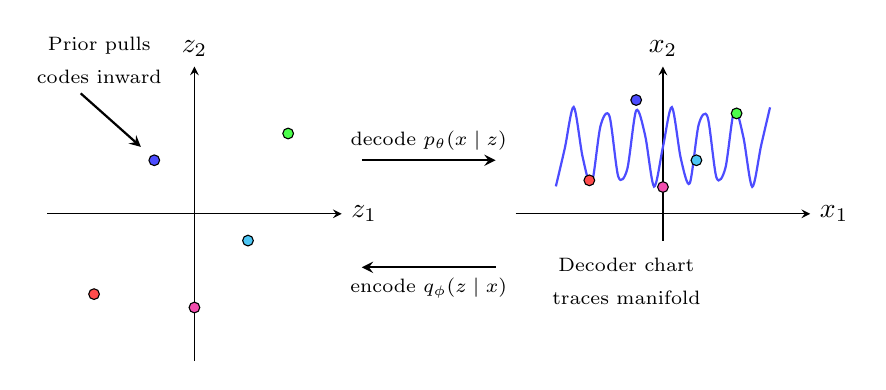
\begin{tikzpicture}[scale=0.85, >=stealth]
        % Latent space axes
        \begin{scope}
            \draw[->] (-2.2,0) -- (2.2,0) node[right] {$z_1$};
            \draw[->] (0,-2.2) -- (0,2.2) node[above] {$z_2$};
            % \node at (0,2.5) {\small Latent space $z$};
            \foreach \x/\y/\c in { -1.5/-1.2/red, -0.6/0.8/blue, 0.8/-0.4/cyan, 1.4/1.2/green, 0.0/-1.4/magenta} {
                \filldraw[fill=\c!70, draw=black] (\x,\y) circle (0.08);
            }
            \draw[->, thick] (-1.7,1.8) -- (-0.8,1.0);
            \node[align=center, anchor=south west] at (-2.5,1.8) {\scriptsize Prior pulls\\\scriptsize codes inward};
        \end{scope}
        % Decoder arrow
        \draw[->, thick] (2.5,0.8) -- (4.5,0.8) node[midway, above] {\scriptsize decode $p_\theta(x\mid z)$};
        % Data manifold axes
        \begin{scope}[xshift=7cm]
            \draw[->] (-2.2,0) -- (2.2,0) node[right] {$x_1$};
            \draw[->] (0,-0.4) -- (0,2.2) node[above] {$x_2$};
            % \node at (0,2.5) {\small Data manifold in $x$};
            % Manifold curve
            \draw[thick, blue!70] plot [smooth, domain=-1.6:1.6] (\x,{1 + 0.6*sin(\x r * 60)});
            % Points mapped
            \foreach \x/\y/\c in { -1.1/0.5/red, -0.4/1.7/blue, 0.5/0.8/cyan, 1.1/1.5/green, 0.0/0.4/magenta} {
                \filldraw[fill=\c!70, draw=black] (\x,\y) circle (0.08);
            }
            \node[align=center, anchor=south west] at (-1.8,-1.5) {\scriptsize Decoder chart\\\scriptsize traces manifold};
        \end{scope}
        % Encoder arrow
        \draw[<-, thick] (2.5,-0.8) -- (4.5,-0.8) node[midway, below] {\scriptsize encode $q_\phi(z\mid x)$};
    \end{tikzpicture}
    \caption{The encoder learns manifold coordinates while the decoder maps latent points back onto the curved data manifold, keeping interpolations smooth.}
    \label{fig:vae_manifold}
\end{figure}

\subsection{A Bayesian detour}
Bayesian estimation provides intuition for why priors help disentangle noise from signal. Suppose we wish to estimate the mean shoe size $\mu$ in a small town. A Gaussian prior $\mu \sim \mathcal N(\alpha, \beta)$ captures our belief before collecting data. Observing measurements $x_1, \ldots, x_n$ with $x_i \sim \mathcal N(\mu, 1)$ yields a Gaussian posterior $\mathcal N(\mu \mid m, s^2)$ that balances the prior and the evidence. When few samples are available, the posterior stays near $\alpha$ (robustness to noise); as $n$ grows, the data dominate (informativeness). VAEs apply the same logic in every latent dimension: the prior $p(z)$ nudges encodings toward structured, disentangled regions while still allowing the decoder to reconstruct the input accurately.

\section{Non-parametric Bayesian Methods}

How can we endow probabilistic models with enough flexibility to grow with the data instead of committing to a fixed number of parameters? Non-parametric Bayesian methods answer this question by replacing finite-dimensional priors with distributions over infinite-dimensional objects such as probability measures. This chapter traces the path from Bayesian inference for a single Gaussian to Gaussian mixture models (GMMs) with an unbounded number of clusters, highlighting the role of conjugate priors, Gibbs sampling, Dirichlet processes, and exchangeability.

\subsection{Warm-up: Bayesian inference for a single Gaussian}
Consider one-dimensional observations $X = \{x_1, \ldots, x_n\}$ drawn i.i.d.\ from $\mathcal N(\mu, \sigma^2)$ with known variance $\sigma^2=1$ but unknown mean $\mu$. Bayesians update a prior belief $\mu \sim \mathcal N(m_0, k_0^{-1})$ via Bayes' rule:
\[
p(\mu \mid X) \propto p(X \mid \mu) \, p(\mu) = \left( \prod_{i=1}^n \mathcal N(x_i \mid \mu, 1)\right) \mathcal N(\mu \mid m_0, k_0^{-1}).
\]
Because Gaussians are conjugate to themselves, the posterior remains Gaussian with parameters
\[
m_n = \frac{k_0 m_0 + n \bar x}{k_0 + n}, \qquad k_n = k_0 + n,
\]
where $\bar x$ is the sample mean. Intuitively, $k_0$ quantifies how confident we were in $m_0$; after seeing $n$ data points, the precision simply adds up. The posterior mean $m_n$ is a weighted average between the prior mean and the data mean, showcasing regularization against outliers and a principled notion of uncertainty.

\subsection{Multivariate Gaussians and conjugate priors}
For $d$-dimensional data $x_i \sim \mathcal N(\mu, \Sigma)$ with both $\mu$ and $\Sigma$ unknown, the normal-inverse-Wishart (NIW) distribution is a conjugate prior whose hyperparameters carry clear meaning: 
\begin{itemize}
    \item $m_0 \in \mathbb{R}^d$: prior mean vector,
    \item $k_0 > 0$: scaling factor controlling confidence in $m_0$,
    \item $S_0 \in \mathbb{R}^{d \times d}$: scale matrix encoding prior beliefs about covariance structure,
    \item $\nu_0 > d - 1$: degrees of freedom, controlling confidence in $S_0$.
\end{itemize}
Crucially, the inverse-Wishart component enforces that sampled covariance matrices remain positive semi-definite, which is required for any valid multivariate Gaussian. The NIW density is
\[
p(\mu, \Sigma) = \operatorname{NIW}(\mu, \Sigma \mid m_0, k_0, S_0, \nu_0).
\]
Given a dataset $X$, Bayes' rule yields the posterior
\[
p(\mu, \Sigma \mid X) = \operatorname{NIW}(m_n, k_n, S_n, \nu_n),
\]
with updates
\[
\begin{aligned}
k_n &= k_0 + n, \qquad &\nu_n &= \nu_0 + n,\\
m_n &= \frac{k_0 m_0 + n \bar x}{k_0 + n}, \qquad &S_n &= S_0 + S_X + \frac{k_0 n}{k_0 + n} (\bar x - m_0)(\bar x - m_0)^\top,
\end{aligned}
\]
where $S_X$ is the sample covariance matrix. Only sufficient statistics (mean and covariance) are required, making posterior updates computationally light even for large $n$.

\subsection{Sampling with semi-conjugate priors}
Fully conjugate priors are convenient but sometimes too rigid—for instance, we may want to express separate beliefs about the location and spread of the data. Under an NIW prior the strength of the prior mean and the tightness of the covariance are linked through $k_0$, so tightening one automatically tightens the other. Semi-conjugate priors break this coupling while keeping \emph{conditionally} conjugate updates, which is all Gibbs sampling needs. A typical choice specifies
\[
\mu \sim \mathcal N(m_0, V_0), \qquad \Sigma \sim \operatorname{IW}(S_0, \nu_0),
\]
so the joint density no longer has a closed form but the conditional posteriors do. The
Given current samples, Gibbs sampling iterates:
\[
\mu \mid \Sigma, X \sim \mathcal{N}\left(m_p, V_p\right)
\]
\[
\Sigma \mid \mu, X \sim \operatorname{IW}\left(S_p, v_p\right)
\]
Each step has the same flavor as the fully conjugate update: the data provide sufficient statistics, while the prior contributes virtual observations. Even though the joint posterior $p(\mu, \Sigma \mid X)$ cannot be written explicitly, the Markov chain that alternates these two conditional draws converges to it under mild conditions. Practical samplers further exploit graphical- model independencies (via d-separation) and Rao-Blackwellization to reduce variance and shorten burn-in.

\paragraph{Gibbs sampler details.}
A single Gibbs sweep for this semi-conjugate model proceeds as follows:
\begin{enumerate}
    \item Given the current covariance sample $\Sigma^{(t)}$, draw a new mean by sampling $\mu^{(t+1)}$ from the Gaussian conditional above (using $\Sigma^{(t)}$ inside the formula).
    \item Plug $\mu^{(t+1)}$ into the inverse-Wishart conditional to draw the next covariance sample $\Sigma^{(t+1)}$.
    \item Repeat these two steps for many iterations, discarding the first $T_{\text{burn}}$ draws as burn-in and optionally thinning the remainder.
\end{enumerate}
Because each conditional depends on the latest value of the other block, the chain ``zig-zags'' through the $(\mu, \Sigma)$ space but still converges to the true joint posterior. Conditional independence structure (e.g., between clusters in a mixture) allows updating blocks in parallel or integrating out nuisance variables before running the sampler.

\begin{figure}[ht]
    \centering
    \includegraphics[width=0.6\textwidth]{images/gibbs.png}
    \caption{Gibbs sampling illustration.}
    \label{fig:gibbs_sampling}
\end{figure}

\subsection{Gibbs sampling in a nutshell}
Whenever the posterior $p(\Theta \mid X)$ factorizes into conditionals that are easy to sample from, \emph{Gibbs sampling} provides a route to approximate inference even if the joint density is intractable. Let $\Theta = (\Theta_1, \ldots, \Theta_\ell)$ be the latent variables of interest. Gibbs sampling constructs a Markov chain $\{\Theta^{(t)}\}_{t=0}^\infty$ by iterating:
\begin{enumerate}
    \item Initialize $\Theta^{(0)}$ arbitrarily (e.g., random cluster assignments).
    \item For $t = 0,1,2,\ldots$:
    \begin{enumerate}
        \item Sample $\Theta_1^{(t+1)} \sim p(\Theta_1 \mid \Theta_2^{(t)}, \ldots, \Theta_\ell^{(t)}, X)$.
        \item Sample $\Theta_2^{(t+1)} \sim p(\Theta_2 \mid \Theta_1^{(t+1)}, \Theta_3^{(t)}, \ldots, \Theta_\ell^{(t)}, X)$.
        \item Continue cycling through all coordinates until $\Theta_\ell^{(t+1)}$ is sampled given the most recent values of the others.
    \end{enumerate}
\end{enumerate}
Each conditional draw is typically conjugate (or otherwise tractable) because all variables except one are held fixed. Under mild regularity conditions this Markov chain has $p(\Theta \mid X)$ as its stationary distribution, so samples collected after a burn-in period approximate the true posterior. In practice we discard the first $T_\text{burn}$ iterations, then thin or average the remaining ones to estimate expectations. The method shines in models such as GMMs where conditionals like $p(z_i \mid z_{-i}, \pi, \mu, \Sigma, X)$ or $p(\mu_k, \Sigma_k \mid z, X)$ admit closed forms.

\begin{figure}[ht]
    \centering
    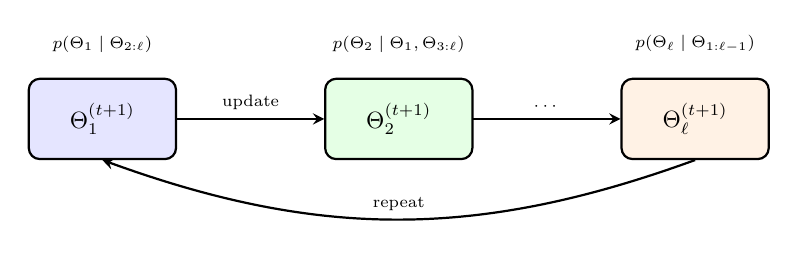
\begin{tikzpicture}[node distance=2.2cm, >=stealth, thick, scale=0.85, every node/.style={transform shape}]
        \node[draw, rounded corners, fill=blue!10, minimum width=2.2cm, minimum height=1.2cm] (thetaone) {$\Theta_1^{(t+1)}$};
        \node[draw, rounded corners, fill=green!10, minimum width=2.2cm, minimum height=1.2cm, right=of thetaone] (thetatwo) {$\Theta_2^{(t+1)}$};
        \node[draw, rounded corners, fill=orange!10, minimum width=2.2cm, minimum height=1.2cm, right=of thetatwo] (thetak) {$\Theta_\ell^{(t+1)}$};
        \node[above=0.25cm of thetaone] {\scriptsize $p(\Theta_1 \mid \Theta_{2:\ell})$};
        \node[above=0.25cm of thetatwo] {\scriptsize $p(\Theta_2 \mid \Theta_{1},\Theta_{3:\ell})$};
        \node[above=0.25cm of thetak] {\scriptsize $p(\Theta_\ell \mid \Theta_{1:\ell-1})$};
        \draw[->] (thetaone) -- node[above] {\scriptsize update} (thetatwo);
        \draw[->] (thetatwo) -- node[above] {\scriptsize $\cdots$} (thetak);
        % \draw[->, bend left=40] (thetak.north east) to node[above] {\scriptsize $t+1 \rightarrow t+2$} ([yshift=0.5cm]thetaone.north west);
        \draw[->, bend left=20] (thetak.south) to  node[above] {\scriptsize repeat} (thetaone.south);
    \end{tikzpicture}
    \caption{Gibbs Sampling}
    \label{fig:gibbs_cycle}
\end{figure}

% Rest is not part of the exam

% \subsection{Bayesian inference for finite Gaussian mixtures}
% A $K$-component GMM introduces latent labels $z_i \in \{1, \ldots, K\}$ and cluster-specific parameters $(\mu_k, \Sigma_k)$ with mixing proportions $\pi_k$. A standard Bayesian specification is
% \[
% \begin{aligned}
% \pi &\sim \operatorname{Dir}(\alpha_0, \ldots, \alpha_0),\\
% \mu_k, \Sigma_k &\sim \operatorname{NIW}(m_0, k_0, S_0, \nu_0), \qquad k=1,\ldots,K,\\
% z_i \mid \pi &\sim \operatorname{Categorical}(\pi),\\
% x_i \mid z_i, \{\mu_k, \Sigma_k\} &\sim \mathcal N(\mu_{z_i}, \Sigma_{z_i}).
% \end{aligned}
% \]
% Gibbs sampling alternates between:
% \begin{enumerate}
%     \item Sampling cluster assignments $z_i$ given $\pi$ and current Gaussian parameters. Using Bayes' rule and d-separation, the conditional is proportional to
%     \[
%     p(z_i = k \mid z_{-i}, \pi, X, \{\mu_k, \Sigma_k\}) \propto \pi_k \, \mathcal N(x_i \mid \mu_k, \Sigma_k).
%     \]
%     \item Sampling $\pi$ from its conditional Dirichlet distribution with counts $n_k$.
%     \item Sampling each $(\mu_k, \Sigma_k)$ from the NIW posterior conditioned on points assigned to cluster $k$.
% \end{enumerate}
% The strong coupling between parameters and labels, however, can slow mixing. Collapsed Gibbs sampling marginalizes out $\pi, \mu_k, \Sigma_k$ analytically using conjugacy, yielding more efficient sampling over $\{z_i\}$ alone. Rao-Blackwell's theorem guarantees that such marginalization reduces estimator variance compared to sampling all variables explicitly.

% \subsection{From fixed to unbounded clusters}
% Setting $K$ requires prior knowledge and often leads to either underfitting (if $K$ is too small) or overfitting (if $K$ is too large). Non-parametric Bayesian modeling removes this bottleneck by allowing a potentially infinite number of clusters, yet ensuring that only finitely many are used for any finite dataset. The Dirichlet process (DP) is the key ingredient. Formally, a DP with base distribution $H$ and concentration $\alpha>0$ is a distribution over probability measures $G$ such that for any measurable partition $(T_1, \ldots, T_m)$ of the sample space,
% \[
% (G(T_1), \ldots, G(T_m)) \sim \operatorname{Dir}(\alpha H(T_1), \ldots, \alpha H(T_m)).
% \]
% Draws from a DP are discrete with probability one, making them ideal priors over mixture weights when the number of components is unknown.

% \subsection{Chinese restaurant process intuition}
% The \emph{Chinese restaurant process} (CRP) is a distribution over partitions that emerges when integrating out the random measure $G$ in a DP mixture model. Imagine customers (data points) entering a restaurant with infinitely many tables (clusters). The $i$-th customer sits at an occupied table $k$ with probability proportional to the number $n_k$ of customers already there, or starts a new table with probability proportional to $\alpha$:
% \[
% p(z_i = k \mid z_{1:i-1}) =
% \begin{cases}
% \frac{n_k}{\alpha + i - 1}, & \text{existing table } k,\\[4pt]
% \frac{\alpha}{\alpha + i - 1}, & \text{new table}.
% \end{cases}
% \]
% This simple rule balances reinforcement (popular tables attract more customers) with innovation controlled by $\alpha$. The expected number of occupied tables after $n$ customers is $\mathcal O(\alpha \log n)$, ensuring growth is sublinear in the data size.

% \subsection{Dirichlet process Gaussian mixtures}
% Combining the CRP prior over partitions with Gaussian emission distributions yields the Dirichlet process Gaussian mixture model (DP-GMM). One generative story proceeds as follows:
% \begin{enumerate}
%     \item Draw mixture weights $G \sim \operatorname{DP}(\alpha, H)$, where $H$ is typically the NIW prior over Gaussian parameters.
%     \item For each cluster, draw $(\mu_k, \Sigma_k) \sim H$.
%     \item For each datapoint, sample a cluster index $\theta_i \sim G$ and then $x_i \sim \mathcal N(\mu_{\theta_i}, \Sigma_{\theta_i})$.
% \end{enumerate}
% Integrating out $G$ induces CRP-style probabilities over the $\theta_i$.

% Collapsed Gibbs sampling for a DP-GMM mirrors the finite case but replaces the multinomial counts with the CRP partition structure. Specifically, the conditional distribution of $z_i$ given the other assignments and data is proportional to:
% \[
% p(z_i = k \mid z_{-i}, X) \propto
% \begin{cases}
% (n_{k,-i})\, p(x_i \mid X_{k,-i}) & \text{existing cluster } k,\\[4pt]
% \alpha \int p(x_i \mid \theta) \, H(d\theta) & \text{new cluster,}
% \end{cases}
% \]
% where $p(x_i \mid X_{k,-i})$ is the posterior predictive under cluster $k$ with $x_i$ excluded. The second term—the integral over the base measure—has a closed-form expression under conjugate choices (e.g., NIW), making sampling practical.

% \subsection{Stick-breaking construction}
% An alternative perspective on the DP is the stick-breaking process. Draw independent $v_k \sim \operatorname{Beta}(1, \alpha)$ and define weights
% \[
% \pi_k = v_k \prod_{j<k} (1 - v_j), \qquad k = 1, 2, \ldots
% \]
% The weights sum to one almost surely, resembling the act of repeatedly breaking off a random fraction of a unit-length stick. The stick-breaking view clarifies how the concentration parameter $\alpha$ affects sparsity: small $\alpha$ leads to a few large weights, while large $\alpha$ spreads mass over many components.

% \subsection{Exchangeability and De Finetti's theorem}
% Although CRP assignments are not independent, they are exchangeable: any permutation of the order in which customers arrive yields the same joint distribution. De Finetti's theorem explains this phenomenon by stating that exchangeable sequences are mixtures of i.i.d.\ sequences. In the DP-GMM context, the latent measure $G$ plays the role of the mixing measure; conditioning on $G$ makes the $\theta_i$ i.i.d. This viewpoint legitimizes the CRP as a consistent prior over partitions and ensures that posterior inference does not depend on the arbitrary ordering of data.

% \subsection{Putting it all together}
% Non-parametric Bayesian methods extend the strengths of finite Bayesian models—uncertainty quantification, principled regularization, and compatibility with probabilistic programming—to scenarios where capacity must adapt to data complexity. The workflow is:
% \begin{enumerate}
%     \item Specify conjugate base measures (e.g., NIW for Gaussian emissions) to keep posterior predictives tractable.
%     \item Use collapsed Gibbs sampling to integrate out nuisance parameters and sample only the essential latent variables (cluster assignments). Rao-Blackwellization reduces variance and accelerates convergence.
%     \item Interpret the resulting assignments through the lens of the CRP or stick-breaking to understand how $\alpha$ influences cluster proliferation.
%     \item Leverage exchangeability to justify that inferences do not depend on data ordering, paving the way for streaming variants.
% \end{enumerate}
% The result is a flexible model that discovers the appropriate number of clusters on the fly, resists overfitting by sharing statistical strength through priors, and retains the interpretability of Bayesian posteriors over both parameters and structure.

\include{18 Probably Approximately Correct Learning}

%\bibliographystyle{alpha}
%\bibliography{sample}

\end{document}
